\documentclass{article}

\input{~/projects/latex/dist/full.tex}

\usepackage{lmodern}
\usepackage{pgfplots}
\setFontType{sans}

\renewcommand{\authorTitle}{Robin Bacher, Janis Hutz\\\url{https://github.com/janishutz/eth-summaries}}
\renewcommand{\authorHeaders}{Robin Bacher, Janis Hutz}
\setLang{de}

\setup{Numerical Methods for Computer Science}
\newcommand{\innumpy}{\fhlc{Cyan}{In \texttt{numpy}}\smallhspace}

\begin{document}
\startDocument
\usetcolorboxes
\setNumberingStyle{3}
\setSubsectionNumbering{1}

%          ╭────────────────────────────────────────────────╮
%          │                   Title page                   │
%          ╰────────────────────────────────────────────────╯
\vspace{2cm}
\begin{center}
    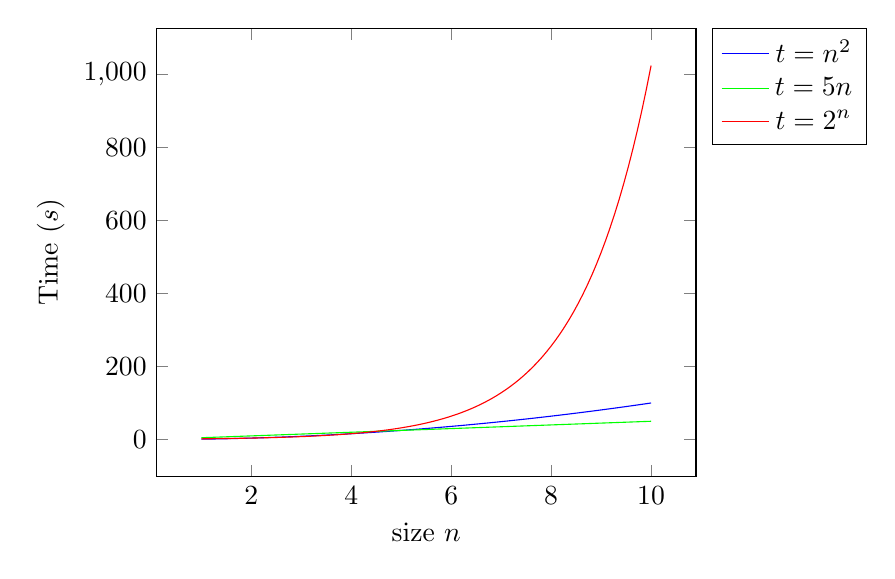
\begin{tikzpicture}
        \begin{axis}[
                legend pos=outer north east,
                axis lines = box,
                xlabel = size $n$,
                ylabel = Time ($s$),
                variable = t,
                trig format plots = rad,
            ]
            \addplot [
                domain=1:10,
                samples=100,
                color=blue,
            ]
            {x^2};
            \addlegendentry{$t = n^2$}
            \addplot [
                domain=1:10,
                samples=100,
                color=green,
            ]
            {5 * x};
            \addlegendentry{$t = 5n$}
            \addplot [
                domain=1:10,
                samples=100,
                color=red,
            ]
            {2^x};
            \addlegendentry{$t = 2^n$}
        \end{axis}
    \end{tikzpicture}
\end{center}



\vspace{3cm}
\begin{center}
    \begin{Large}
        \quote{Wenn ich keine Lust habe, das zu berechnen, dann wende ich einfach Gewalt an}
    \end{Large}

    \hspace{3cm} - Prof. Dr. Vasile Gradinaru, 2025
\end{center}

\vspace{2cm}
\begin{center}
    HS2025, ETHZ\\[0.2cm]
    \begin{Large}
        Summary of the Script and Lectures
    \end{Large}\\[0.2cm]
\end{center}


% ────────────────────────────────────────────────────────────────────

%          ╭────────────────────────────────────────────────╮
%          │               Table of Contents                │
%          ╰────────────────────────────────────────────────╯
\newpage
\printtoc{ForestGreen}


% ────────────────────────────────────────────────────────────────────

%          ╭────────────────────────────────────────────────╮
%          │                  Introduction                  │
%          ╰────────────────────────────────────────────────╯
\newpage
\setcounter{section}{-1}
\section{Introduction}
This summary is intended to give you a broad overview of the topics relevant for the exam.
While it aims to serve as a full on replacement for the script, please do not fully rely on it, as there may be mistakes, inaccuracies and missing details as compared to the script.
Furthermore, you will only have access to the script during the exam, so getting familiar with the script is a good idea.
We have decided to write it in German, as is the new script and for some of the topics that are poorly explained in the script, we have added further explanations.

The numbering should match the script's numbering exactly (apart from the cases where two definitions were combined due to being closely related and short),
making it easier for you to look up the relevant definitions, theorems, etc in context in the script.

Many of the figures in this summary were taken directly from the Script or Lecture notes created by Professor Vasile Gradinaru.

We have also taken some explanations and code examples from the slides of our TA, Nils Müller, whose slides can be found
\hlhref{https://n.ethz.ch/~muellerni/courses/numcs25.php}{here}. (Link will be updated if we are to get a new website link from him, as n.ethz.ch is down now)
% TODO: Update this when n.ethz is taken offline completely

A few things to be familiar with for the exam to be quicker at solving exercises:
\begin{itemize}
    \item The script. You do not have to know basically anything by heart, so knowing where to find things in the script quickly (and knowing quirks of naming in the script)
          will make you much quicker. When searching, always use as short of a keyword as possible while not having hundreds of results.
    \item Be aware that some things might not be called the same way they are in the script in the exercises.
          If you don't find it immediately, go to the appropriate section in the script (using the index in the PDF reader (that is likely PDF.js, Firefox's PDF reader))
          and manually search for it there.
    \item Get familiar with the concepts that \texttt{NumPy} uses (i.e. how to do slicing, etc). See section \ref{sec:python} for an overview over some of the concepts.
    \item Learn the basics of \texttt{Sympy}, as that will spare you having to do integrals. See section \ref{sec:sympy} for an introduction to \texttt{Sympy}.
\end{itemize}

\fhlc{Cyan}{Code Examples}

We tried to add short and easily understandable code examples wherever possible.\\
Complete code (with many visualisations), also for topics not covered in this summary, can be found \hlhref{https://github.com/RobinB27/numcs25}{here}.

% ────────────────────────────────────────────────────────────────────

%          ╭────────────────────────────────────────────────╮
%          │                  Main content                  │
%          ╰────────────────────────────────────────────────╯

% ── Introduction ────────────────────────────────────────────────────
\newsection
\section{Einführung}
% ┌                                                ┐
% │     AUTHOR: Janis Hutz<info@janishutz.com>     │
% └                                                ┘

\subsection{Rundungsfehler}

\begin{definition}[]{Absoluter \& Relativer Fehler}
    \begin{multicols}{2}
        \begin{itemize}
            \item \bi{Absoluter Fehler}: $||\tilde{x} - x||$
            \item \bi{Relativer Fehler}: $\displaystyle \frac{||\tilde{x} - x||}{||x||}$ für $||x|| \neq 0$
        \end{itemize}
    \end{multicols}
    wobei $\tilde{x}$ eine Approximation an $x \in \R$ ist
\end{definition}

Rundungsfehler entstehen durch die (verhältnismässig) geringe Präzision die man mit der Darstellung von Zahlen auf Computern erreichen kann.
Zusätzlich kommt hinzu, dass durch Unterläufe (in diesem Kurs ist dies eine Zahl die zwischen $0$ und der kleinsten darstellbaren, positiven Zahl liegt) Präzision verloren gehen kann.

Überläufe hingegen sind konventionell definiert, also eine Zahl, die zu gross ist und nicht mehr dargestellt werden kann.


\setcounter{all}{9}
\begin{remark}[]{Auslöschung}
    Bei der Subtraktion von zwei ähnlich grossen Zahlen kann es zu einer Addition der Fehler der beiden Zahlen kommen, was dann den relativen Fehler um einen sehr grossen Faktor vergrössert.
    Die Subtraktion selbst hat einen vernachlässigbaren Fehler
\end{remark}

\setcounter{all}{18}
\fancyex{Ableitung mit imaginärem Schritt} Als Referenz in Graphen wird hier oftmals die Implementation des Differenzialquotienten verwendet.

Der Trick hier ist, dass wir mit Komplexen Zahlen in der Taylor-Approximation einer glatten Funktion in $x_0$ einen rein imaginären Schritt durchführen können:
\begin{align*}
    f(x_0 + ih) = f(x_0) + f'(x_0)ih - \frac{1}{2} f''(x_0)h^2 - iC \cdot h^3 \text{ für } h \in \R \text{ und } h \rightarrow 0
\end{align*}
Da $f(x_0)$ und $f''(x_0)h^2$ reell sind, verschwinden die Terme, wenn wir nur den Imaginärteil des Ausdruckes weiterverwenden. Nach weiteren Vereinfachungen und Umwandlungen erhalten wir
\begin{align*}
    f'(x_0) \approx \frac{\text{Im}(f(x_0 + ih))}{h}
\end{align*}

Falls jedoch hier die Auswertung von $\text{Im}(f(x_0 + ih))$ nicht exakt ist, so kann der Fehler beträchtlich sein.


\setcounter{all}{20}
\fancyex{Konvergenzbeschleunigung nach Richardson}
\begin{align*}
    y f'(x) & = y d\left(\frac{h}{2}\right) + \frac{1}{6} f'''(x) h^2 + \frac{1}{480}f^{(s)} h^4 + \ldots - f'(x) \\
            & = -d(h) - \frac{1}{6}f'''(x) h^2 + \frac{1}{120} f^{(s)}(x) h^n \Leftrightarrow 3 f'(x)             \\
            & = 4 d\left(\frac{h}{2}\right)  d(h) + \tco{h^4} \Leftrightarrow
\end{align*}
% TODO: Need to finish with notes from the exercise sessions


\fhlc{Cyan}{Schema}

\begin{align*}
    d(h) = \frac{f(x + h) - f(x - h)}{2h}
\end{align*}

wobei im Schema dann
\begin{align*}
    R_{l, 0} = d\left( \frac{h}{2^l} \right)
\end{align*}
und
\begin{align*}
    R_{l, k} = \frac{4^k \cdot R_{l, k - 1} - R_{l - 1, k - 1}}{4^k - 1}
\end{align*}
und $f'(x) = R_{l, k} + C \cdot \left( \frac{h}{2^l} \right)^{2k + 2}$

% ┌                                                ┐
% │     AUTHOR: Janis Hutz<info@janishutz.com>     │
% └                                                ┘

\newsection
\subsection{Rechenaufwand}
In NumCS wird die Anzahl elementarer Operationen wie Addition, Multiplikation, etc benutzt, um den Rechenaufwand zu beschreiben. 
Wie in Algorithmen und * ist auch hier wieder $\tco{\ldots}$ der Worst Case.
Teilweise werden auch andere Funktionen wie $\sin, \cos, \sqrt{\ldots}, \ldots$ dazu gezählt.

Die Basic Linear Algebra Subprograms (= BLAS), also grundlegende Operationen der Linearen Algebra, wurden bereits stark optimiert und sollten wann immer möglich verwendet werden und man sollte auf keinen Fall diese selbst implementieren.

Dieser Kurs verwendet \texttt{numpy}, \texttt{scipy}, \texttt{sympy} (collection of implementations for symbolic computations) und \texttt{matplotlib}.
Dieses Ecosystem ist eine der Stärken von Python und ist interessanterweise zu einem Grossteil nicht in Python geschrieben, da dies sehr langsam wäre.

% ┌                                                ┐
% │     AUTHOR: Janis Hutz<info@janishutz.com>     │
% └                                                ┘

\newsection
\subsection{Rechnen mit Matrizen}
Wie in Lineare Algebra besprochen, ist das Resultat der Multiplikation einer Matrix $A \in \C^{m \times n}$ und einer Matrix $B \in \C^{n \times p}$ ist eine Matrix $AB = \in \C^{m \times p}$

\innumpy haben wir folgende Funktionen:
\begin{itemize}
    \item \verb|b @ a| (oder \verb|np.dot(b, a)| oder \verb|np.einsum('i,i', b, a)| für das Skalarprodukt
    \item \verb|A @ B| (oder \verb|np.einsum('ik,kj->ij', )|) für das Matrixprodukt
    \item \verb|A @ x| (oder \verb|np.einsum('ij,j->i', A, x)|) für Matrix $\times$ Vektor
    \item \verb|A.T| für die Transponierung
    \item \verb|A.conj()| für die komplexe Konjugation (kombiniert mit \verb|.T| = Hermitian Transpose)
    \item \verb|np.kron(A, B)| für das Kroneker Produkt
    \item \verb|b = np.array([4.j, 5.j])| um einen Array mit komplexen Zahlen zu erstellen (\verb|j| ist die imaginäre Einheit, aber es muss eine Zahl direkt daran geschrieben werden)
\end{itemize}


\setLabelNumber{all}{4}
\fancyremark{Rang der Matrixmultiplikation} $\text{Rang}(AX) = \min(\text{Rang}(A), \text{Rang}(X))$

\setLabelNumber{all}{7}
\fancyremark{Multiplikation mit Diagonalmatrix $D$} $D \times A$ skaliert die Zeilen von $A$ während $A \times D$ die Spalten skaliert

\stepcounter{all}
\inlineex \verb|D @ A| braucht $\tco{n^3}$ Operationen, wenn wir jedoch \verb|D.diagonal()[:, np.newaxis] * A| verwenden, so haben wir nur noch $\tco{n^2}$ Operationen, da wir die vorige Bemerkung Nutzen und also nur noch eine Skalierung vornehmen.
So können wir also eine ganze Menge an Speicherzugriffen sparen, was das Ganze bedeutend effizienter macht

\setLabelNumber{all}{14}
\inlineremark Wir können bestimmte Zeilen oder Spalten einer Matrix skalieren, in dem wir einer Identitätsmatrix im unteren Dreieck ein Element hinzufügen.
Wenn wir nun diese Matrix $E$ (wie die in der $LU$-Zerlegung) linksseitig mit der Matrix $A$ multiplizieren (bspw. $E^{(2, 1)}A$), dann wird die zugehörige Zeile skaliert.
Falls wir aber $AE^{(2, 1)}$ berechnen, so skalieren wir die Spalte

\fancyremark{Blockweise Berechnung} Man kann das Matrixprodukt auch Blockweise berechnen.
Dazu benutzen wir eine Matrix, deren Elemente andere Matrizen sind, um grössere Matrizen zu generieren.
Die Matrixmultiplikation funktioniert dann genau gleich, nur dass wir für die Elemente Matrizen und nicht Skalare haben.

% ────────────────────────────────────────────────────────────────────
\hspace{1mm}
\hrule
\hspace{1mm}
Untenstehend eine Tabelle zum Vergleich der Operationen auf Matrizen

\begin{tables}{lcccc}{Name           & Operation & Mult  & Add         & Komplexität}
              Skalarprodukt          & $x^H y$   & $n$   & $n - 1$     & $\tco{n}$    \\
              Tensorprodukt          & $x y^H$   & $nm$  & $0$         & $\tco{mn}$   \\
              Matrix $\times$ Vektor & $Ax$      & $mn$  & $(n - 1)m$  & $\tco{mn}$   \\
              Matrixprodukt          & $AB$      & $mnp$ & $(n - 1)mp$ & $\tco{mnp}$  \\
\end{tables}
\inlineremark Das Matrixprodukt kann mit Strassen's Algorithmus mithilfe der Block-Partitionierung in $\tco{n^{\log_2(7)}} \approx \tco{n^{2.81}}$ berechnet werden.

\fancyremark{Rang 1 Matrizen} Können als Tensorprodukt von zwei Vektoren geschrieben werden.
Dies ist beispielsweise hierzu nützlich:

Sei $A = ab^\top$. Dann gilt $y = Ax \Leftrightarrow y = a(b^\top x)$, was dasselbe Resultat ergibt, aber nur $\tco{m + n}$ Operationen und nicht $\tco{mn}$ benötigt wie links.

\inlineex Für zwei Matrizen $A, B \in \R^{n \times p}$ mit geringem Rang $p \ll n$, dann kann mithilfe eines Tricks die Rechenzeit von \verb|np.triu(A @ B.T) @ x| von $\tco{pn^2}$ auf $\tco{pn}$ reduziert werden.
Die hier beschriebene Operation berechnet $\text{Upper}(AB^\top) x$ wobei $\text{Upper}(X)$ das obere Dreieck der Matrix $X$ zurück gibt.
Wir nennen diese Matrix hier $R$.

\innumpy können wir den folgenden Ansatz verwenden, um die Laufzeit zu verringern:
Da die Matrix $R$ eine obere Dreiecksmatrix ist, ist das Ergebnis die Teilsummen von unserem Umgekehrten Vektor $x$,
also können wir mit \verb|x[::-1].cumsum(axis=0)[::-1]| die Kummulative Summe berechnen.
Das \verb|[::-1]| dient hier lediglich dazu, den Vektor $x$ umzudrehen, sodass das richtige Resultat entsteht und die \texttt{axis=0} muss nur spezifiziert werden,
falls wir nicht den Default von \texttt{None} wollen, welcher die \texttt{cumsum} auf \texttt{x.flat} ausführt.
Die vollständige Implementation sieht so aus:
\begin{code}{python}
    def low_rank_matrix_vector_product(A: np.ndarray, B: np.ndarray, x: np.ndarray):
        n = A.shape[0]
        y = np.zeros(n) # Results vector

        # Compute B * x with broadcasting (x needs to be reshaped to 2D)
        v = B * x[:, None]

        # s is defined as the reverse cummulative sum of our vector
        # (and we need it reversed again for the final calculation to be correct)
        s = v[::-1].cumsum(axis=0)[::-1]

        y = np.sum(A * s)
\end{code}


\setLabelNumber{all}{21}
\fancydef{Kronecker-Produkt} Das Kronecker-Produkt ist eine $(ml) \times (nk)$-Matrix, für $A \in \R^{m \times n}$ und $B \in \R^{l \times k}$.

\innumpy können wir dieses einfach mit \verb|np.kron(A, B)| berechnen (ist jedoch nicht immer ideal):
\begin{align*}
    A \otimes B :=
    \begin{bmatrix}
        (A)_{1, 1} B & (A)_{1, 2}B & \ldots & \ldots & (A)_{1, n} B \\
        (A)_{2, 1} B & (A)_{2, 2}B & \ldots & \ldots & (A)_{2, n} B \\
        \vdots       & \vdots      & \ddots & \ddots & \vdots       \\
        (A)_{m, 1} B & (A)_{m, 2}B & \ldots & \ldots & (A)_{m, n} B \\
    \end{bmatrix}
\end{align*}

\fancyex{Multiplikation des Kronecker-Produkts mit Vektor} Wenn man $A \otimes B \cdot x$ berechnet, so ist die Laufzeit $\tco{m \times n \times l \times k}$, aber wenn wir den Vektor $x$ in $n$ gleich grosse Blöcke aufteilen (was man je nach gewünschter nachfolgender Operation in NumPy in $\tco{1}$ machen kann mit \verb|x.reshape(n, x.shape[0] / n)|), dann ist es möglich das Ganze in $\tco{m \cdot l \cdot k}$ zu berechnen.

Die vollständige Implementation ist auch hier nicht schwer und sieht folgendermassen aus:
\begin{code}{python}
    def fast_kron_vector_product(A: np.ndarray, B: np.ndarray, x: np.ndarray):
        # First multiply Bx_i, (and define x_i as a reshaped numpy array to save cost (as that will create a valid array))
        # This will actually crash if x.shape[0] is not divisible by A.shape[0]
        bx = B * x.reshape(A.shape[0], round(x.shape[0] / A.shape[0]))
        # Then multiply a with the resulting vector
        y = A @ bx
\end{code}

Um die oben erwähnte Laufzeit zu erreichen muss erst ein neuer Vektor berechnet werden, oben im Code \verb|bx| genannt, der eine Multiplikation von \verb|Bx_i| als Einträge hat.


% ── polynomial interpolation ────────────────────────────────────────
\newsection
\section{Polynominterpolation}
\newsection
\subsection{Trigonometrische Interpolation}
\subsubsection{Von Approximation zur Interpolation}
Wir erinnern uns daran, dass wir die Fourier-Approximation durch den Abbruch der unendlichen Fourier-Reihe erhalten, oder in anderen Worten, wir verkleinern die Limiten der Summe.

\fancyremark{DFT mit $N = 2n$ Koeffizienten an Punkten $\frac{l}{N}$ für $l = 0, 1, \ldots, N - 1$}

Der Shift ist hier gegeben durch (für $k \geq 0$ ist $\gamma_k = \hat{f}_N(k)$ und für $k < 0$ ist $\gamma_k = \hat{f}_N(N + k)$)
\begin{align*}
    f_{N - 1}(x)                 & = \sum_{k = -n}^{n - 1} \gamma_k e^{2 \pi ikx} = \sum_{k = 0}^{n - 1} \gamma_k e^{2\pi ikx} + \sum_{k = -n}^{-1} \gamma_k e^{2\pi ikx} \\
    \Leftrightarrow f_{N - 1}(x) & = \frac{1}{N} \left( \sum_{j = 0}^{N - 1} \left( f\left( \frac{j}{n} \right)
        \sum_{k = -n}^{n - 1} e^{2\pi ik \left( x - \frac{j}{N} \right)} \right) \right)
\end{align*}

\vspace{-1pc}

Wenn wir die Funktion nun an der Stelle $\frac{l}{N}$ auswerten so erhalten wir:
\rmvspace
\begin{align*}
    f_{N - 1}\left( \frac{l}{N} \right) = \ldots = f\left( \frac{l}{N} \right)
\end{align*}

\vspace{-1.8pc}
was aufgrund der Orthogonalität der diskreten Fourier-Vektoren funktioniert, welche besagt, dass $\displaystyle \sum_{k = -n}^{n - 1} \omega_N^{k(j - l)} = 0$, für alle $j \neq l$.
Für $j = l$ ergibt die Summe $N$.

Dies heisst also, dass die Fourier-Approximation die Interpolationsbedingungen an den Punkten $\frac{l}{N}$ erfüllt,
also können wir die Lösung der Interpolationsaufgabe $p_{N - 1} \left( \frac{l}{N} \right) = f\left( \frac{l}{N} \right)$ f $l = 0, 1, \ldots, N - 1$ im Raum
\rmvspace
\begin{align*}
    \mathcal{T}_N = \text{span}\{ e^{2\pi ijt} \divides j = - \floor{\frac{N - 1}{2}}, \ldots, \floor{\frac{N}{2}} \}
\end{align*}

\rmvspace\rmvspace
folgendermassen finden können: 
\begin{enumerate}[label=(\arabic*)]
    \item Mittels Gleichungssystem $\sum_{j} \gamma_j e^{2\pi ijt_l} = f(t_l)$ für $l = 0, \ldots, N - 1$. Operationen: $\tco{N^3}$
    \item Mittels FFT in $\tco{N \log(N)}$ Operationen, aber nur falls die Punkte äquidistant sind, also $t_l = \frac{l}{N}$.
        Dann ist die Matrix des obigen Gleichungssystems $F^{-1}_N$
\end{enumerate}

\vspace{0.2cm}

Unten findet sich Python code der mit den unterschiedlichen Methoden die Koeffizienten des Trigonometrischen Polynoms bestimmt.
\rmvspace
\begin{code}{python}
    def get_coeff_trig_poly(t: np.ndarray, y: np.ndarray):
    N = y.shape[0]
    if N % 2 == 1:
    n = (N - 1.0) / 2.0
    M = np.exp(2 * np.pi * 1j * np.outer(t, np.arange(-n, n + 1)))
    else:
    n = N / 2.0
    M = np.exp(2 * np.pi * 1j * np.outer(t, np.arange(-n, n)))
    c = np.linalg.solve(M, y)
    return c

    N = 2**12
    t = np.linspace(0, 1, N, endpoint=False)
    y = np.random.rand(N)
    direct = get_coeff_trig_poly(t, y)
    using_fft = np.fft.fftshift(np.fft.fft(y) / N)
    using_ifft = np.conj(np.fft.fftshift(np.fft.ifft(y)))
\end{code}

\subsection{Monombasis}

\fancytheorem{Eindeutigkeit} $p(x) \in \mathcal(P)_k$ ist durch $k+1$ Punkte $y_i = p(x_i)$ eindeutig bestimmt.

Dieser Satz kann direkt angewendet werden zur Interpolation, in dem man $p(x)$ als Gleichungssystem schreibt.
% FIXME: It'd probably be better to use align* environment in general, it's much more flexible
% FIXME: Having a new line before $$ (or align* environment for that matter) makes the space between text and math env larger!
$$
	p_n(x) = \alpha_n x^n + \cdots + \alpha_0 x^0 \quad \iff \quad
	\underbrace{
		\begin{bmatrix}
			1      & x_0    & \cdots & x_0^n  \\
			1      & x_1    & \cdots & x_1^n  \\
			\vdots & \vdots & \ddots & \vdots \\
			1      & x_n    & \cdots & x_n^n  \\
		\end{bmatrix}
	}_\text{Vandermonde Matrix}
	\begin{bmatrix}
		\alpha_0 \\
		\alpha_1 \\
		\vdots   \\
		\alpha_n
	\end{bmatrix}
	=
	\begin{bmatrix}
		y_0    \\
		y_1    \\
		\vdots \\
		y_n
	\end{bmatrix}
$$

Um $\alpha_i$ zu finden ist die Vandermonde Matrix unbrauchbar, da die Matrix schlecht konditioniert ist.

Zur Auswertung von $p(x)$ kann man direkt die Matrix-darstellung nutzen, oder effizienter:

\fancydef{Horner Schema} $p(x) = (x \ldots x ( x (\alpha_n x + \alpha_{n-1}) + \ldots + \alpha_1) + \alpha_0)$

\fhlc{Cyan}{In NumPy} \verb|polyfit| liefert die direkte Auswertung, \verb|polyval| wertet Polynome via Horner-Schema aus. (Gemäss Script, in der Praxis sind diese Funktionen \verb|deprecated|)

\newpage
\subsection{Newton Basis}
% Session: Herleitung unwichtig, konzentrieren auf Funktion/Eigenschaften von Newton/Lagrange.

Die Newton-Basis hat den Vorteil, dass sie leichter erweiterbar als die Monombasis ist.

Die Konstruktion verläuft iterativ, und vorherige Datenpunkte müssen nicht neuberechnet werden.

\begin{align*}
    p_0(x) &= y_0 &\textit{(Anfang: triviales Polynom)} \\
    p_1(x) &= p_0(x) + (x-x_0)\frac{(y_1-y_0)}{(x_1-x_0)} & \textit{(Addition des zweiten Datenpunktes)} \\
    p_2(x) &= p_1(x) + \frac{\frac{(y_2-y_1)}{(x_2-x_1)}-\frac{(y_1-y_0)}{x_1-x_0}}{x_2-x_0} (x-x_0)(x-x_1) & \textit{(Schema lässt sich beliebig weiterführen)}\\
    p_3(x) &= p_2(x) + \ldots
\end{align*}

\setcounter{all}{3}
\fancytheorem{Newton-Basis} $\{ N_0,\ \ldots\ ,N_n\}$ ist eine Basis von $\mathcal{P}_n$
\begin{align*}
    N_0(x) &:= 1 \quad
    N_1(x) := x - x_0 \quad
    N_2(x) := (x-x_0)(x-x_1) \quad \ldots \\
    N_n(x) &:= \prod_{i=0}^{n-1} (x-x_i)
\end{align*}

\subsubsection{Koeffizienten}

Wegen Satz 2.2.3 lässt sich jedes $p_n \in \mathcal{P}_n$ als $p_n(x) =\displaystyle\sum_{i=0}^{n} \beta_i N_i(x)$ darstellen. Ein Gleichungssystem liefert alle $\beta_i$:
\begin{align*}
    \begin{bmatrix}
        1 & 0   & \cdots & 0 \\
        1 & N_0 & \cdots & 0 \\
        \vdots & \vdots & \ddots & \vdots \\
        1 & N_0 & \cdots & N_n
    \end{bmatrix}
    \begin{bmatrix}
        \beta_0 \\
        \beta_1 \\
        \vdots \\
        \beta_n
    \end{bmatrix}
    =
    \begin{bmatrix}
        y_0 \\
        y_1 \\
        \vdots \\
        y_n
    \end{bmatrix}
\end{align*}

Die Matrixmultiplikation in $\mathcal{O}(n^3)$ ist aber nicht nötig: Es gibt ein effizienteres System. 

\setcounter{all}{5}
\fancydef{Dividierte Differenzen} 
\begin{multicols}{2}
    \begin{align*}
        y[x_i] &:= y_i \\
        y[x_i,\ \ldots\ ,x_{i+k}] &\overset{\text{Rec.}}{:=} \frac{y[x_{i+1},\ \ldots\ , x_{i+k}] - y[x_i,\ \ldots\ , x_{i+k-1}]}{x_{i+k}-x_i}
    \end{align*}

    \newcolumn

    \begin{center}
    \begin{tabular}{l|llll}
        $x_0$ & $y[x_0]$ \\
            &          & $>y[x_0,x_1]$        \\
        $x_1$ & $y[x_1]$ &  & $>y[x_0,x_1,x_2]$ \\ 
            &          & $>y[x_1,x_2]$        \\
        $x_2$ & $y[x_2]$ &  & $>y[x_1,x_2,x_3]$ \\
            &          & $>y[x_2,x_3]$        \\
        $x_3$ & $y[x_3]$                        \\
    \end{tabular}
    \end{center}
\end{multicols}

\fancyremark{Äquidistante Stellen}

Falls $x_j = x_0 + \underbrace{j \cdot h}_{:= \Delta^j}$ gilt vereinfacht sich einiges:
\begin{align*}
    y[x_0,x_1] &= \frac{1}{h}\Delta y_0 \\
    y[x_0,x_1,x_2] &= \frac{1}{2!h} \Delta^2 y_0 \\
    y[x_0,\ \ldots\ , x_n] &= \frac{1}{n! h^n} \Delta^n y_0 
\end{align*}

\setcounter{all}{8}
\fancytheorem{Newton} Falls $\beta_j = y[x_0,\ \ldots\ , x_j]$ geht das resultierende Polynom durch alle $(x_i,y_i)$.\\
\footnotesize
(D.h. die dividierten Differenzen sind korrekt.)
\normalsize


\newpage
\begin{multicols}{2}

    Matrixmultiplikation in $\mathcal{O}(n^3)$, Speicher $\mathcal{O}(n^2)$

    \begin{code}{python}
    # Slow matrix approach
    def divdiff_slow(x,y):
        n = y.size
        T = np.zeros((n,n))
        T[:,0] = y

        for l in range(1,n):
            for i in range(n-l):
                T[i, l] = (T[i+1,l-1] - T[i, l-1])
                T[i, l] /= (x[i+l] - x[i])
        
        return T[0,:]
    \end{code}

    \newcolumn

    % Add the vectorized HW solution here

    Vektorisierter Ansatz in $\mathcal{O}(n^2)$, Speicher $\mathcal{O}(n)$

    \begin{code}{python}
    # Fast vectorized approach
    def divdiff_fast(x,y):
        n = y.shape[0]

        for k in range(1, n):
            y[k:] = (y[k:] - y[(k-1):n-1]) 
            y[k:] /= (x[k:] - x[0:n-k])
    
        return y
    \end{code}

\end{multicols}

\subsubsection{Auswertung}

Auswertung eines Newton-Polynoms funktioniert in $\mathcal{O}(n)$ durch ein modifiziertes Horner-Schema:

\begin{multicols}{2}
    
\begin{align*}
    p_0 &:= \beta_n \\
    p_1 &:= (x - x_{n-1})p_0 + \beta_{n-1} \\
    p_2 &:= (x - x_{n-2})p_1 + \beta_{n-2} \\
    \vdots \\
    p_n &= p(x)
\end{align*}

\newcolumn

\begin{code}{python}
    def evalNewton(x_data, beta, x):
        p = np.zeros(x.shape[0])
        p += beta[beta.shape[0]-1]
    
        for i in range(1, n+1):
            p = (x - x_data[n-i])*p + beta[n-i]
      
        return p
\end{code}

\end{multicols}


\subsubsection{Fehler}

\setcounter{all}{11}
\inlinetheorem $f$ $n$-mal diff.-bar, $y_i = f(x_i) \implies \exists \xi \in (\min_i x_i, \max_i x_i)$ s.d. $y[x_0,x_1,\ldots,x_n] = \frac{f^{(n)}(\xi)}{(n+1)!}$

\fancytheorem{Fehler} $f: [a,b] \to \R$ ist $(n+1)$-mal diff.-bar, $p$ ist das Polynom zu $f$ in $x_0,\ldots,x_n \in [a,b]$. 
$$
    \forall x \in [a,b]\ \exists \xi \in (a,b):\quad\quad \underbrace{f(x)-p(x)}_{\text{Fehler}} = \prod_{i=0}^{n}(x-x_i)\cdot\frac{f^{(n+1)}(\xi)}{(n+1)!}
$$

Man bemerke: Die Wahl der Stützpunkte hat direkten Einfluss auf den Fehler.



% ┌                                                ┐
% │     AUTHOR: Janis Hutz<info@janishutz.com>     │
% └                                                ┘

\newsection
\subsection{Lagrange- und Baryzentrische Interpolationsformeln}
% Session: Gemäss TA sehr gut beschrieben im alten Script
\label{sec:barycentric-interpolation}

\begin{definition}[]{Lagrange Polynome}
	Für Knoten (auch gennannt Stützstellen) $x_0, x_1, \ldots, x_n \in \R$ definieren wir die Lagrange-Polynome:
	\begin{align*}
		l_i(x) = \prod_{j = 0 \neq i}^n \frac{x - x_j}{x_i - x_j}
	\end{align*}
\end{definition}
Falls $j = i$ im Produkt, so überspringt $j$ diese Zahl.

\inlineex Seien $x_0, x_1, x_2$ die Stützstellen für die Lagrange-Polynome (mit $n = 2$):
\begin{align*}
	l_0(x) & = \frac{x - x_1}{x_0 - x_1} \cdot \frac{x - x_2}{x_0 - x_2} &
	l_1(x) & = \frac{x - x_0}{x_1 - x_0} \cdot \frac{x - x_2}{x_1 - x_2} &
	l_2(x) & = \frac{x - x_0}{x_2 - x_0} \cdot \frac{x - x_1}{x_2 - x_1}
\end{align*}


\begin{theorem}[]{Lagrange-Interpolationsformel}
	Die Lagrange-Polynome $l_i$ zu den Stützstellen $(x_0, y_0), \ldots, (x_n, y_n)$ bilden eine Basis der Polynome $\mathcal{P}_n$ und es gilt:
	\begin{align*}
		p(x) = \sum_{i = 0}^{n} y_i l_i(x) \text{ mit } l_i(x) = \prod_{j \neq i} \frac{x - x_j}{x_i - x_j}
	\end{align*}
\end{theorem}


\fancyremark{Eigenschaften der Lagrange-Polynome}
\rmvspace
\begin{multicols}{2}
	\begin{enumerate}
		\item $l_i(x_j) = 0 \smallhspace \forall j \neq i$
		\item $l_i(x_i) = 1 \smallhspace \forall i$
		\item $\deg(l_i) = n \smallhspace \forall i$
		\item $\sum_{k = 0}^{n} l_k(x) = 1 \text{ und } \sum_{k = 0}^{n} l_k^{(m)}(x) = 0 \text{ für } m > 0$
	\end{enumerate}
\end{multicols}

Da eine Implementation, welche direkt auf den Lagrange-Polynomen basiert, eine Laufzeit von $\tco{n^3}$ hätte, suchte man nach einer besseren Methode.
Mit der \bi{baryzentrischen Interpolationsformel} wird zuerst ein Pre-Computing auf Teilen der Lagrange-Polynome durchgeführt, was dann dazu führt, dass die Laufzeit auf $\tco{n^2}$ sinkt ($\tco{n}$ für die Auswertung der Formel und $\tco{n^2}$ für die Berechnung der $\lambda_k$).
Man berechnet die baryzentrischen Gewichte $\lambda_k$ folgendermassen:
\rmvspace
\begin{align*}
    \lambda_k = \prod_{j \neq k} \frac{1}{x_k - x_j}
\end{align*}
oder das ganze mithilfe von Numpy:
\begin{code}{python}
    def barycentric_weights(x: np.ndarray) -> np.ndarray:
        n = len(x)
        # Initialize to zeros
        barweight = np.ones(n)
        for k in range(n):
            # Vectorized differences between $x_k$ and all $x$s
            differences = x[k] - x

            # Remove the $k$-th element (and handle edge cases for $k = 0$ and $k = n - 1$)
            if k < n - 1 and k > 0:
                diff_processed = np.concatenate((differences[:k], differences[(k + 1) :]))
                barweight[k] = 1 / np.prod(diff_processed)
            elif k == 0:
                barweight[k] = 1 / np.prod(differences[1:])
            else:
                barweight[k] = 1 / np.prod(differences[:k])
        return barweight
\end{code}

Mit dem können wir dann ein Polynom mit der baryzentrischen Interpolationsformel interpolieren:
\setcounter{numberingConfig}{0}
\begin{formula}[]{Baryzentrische Interpolationsformel}
	\vspace{-1.5pc}
	\begin{align*}
		p(x) = \frac{\displaystyle \sum_{k = 0}^{n} \frac{\lambda_k}{x - x_k} y_k}{\displaystyle \sum_{k = 0}^{n} \frac{\lambda_k}{x - x_k}}
	\end{align*}
\end{formula}
\setcounter{numberingConfig}{3}

Falls wir die Stützstellen als $(n + 1)$ Chebyshev-Abszissen $\displaystyle x_k = \cos\left( \frac{k\pi}{n} \right)$ wählen,
so sind alle $\lambda_k$ gegeben durch $\lambda_k = (-1)^k \delta_k$ mit $\delta_0 = \delta_n = 0.5$ und $\delta_i = 1$.

Mit anderen $\lambda_k$ eröffnet die baryzentrische Formel einen Weg zur Verallgemeinerung der Interpolation mittels rationaler Funktionen und ist entsprechend kein Polynom mehr.

Eine weitere Anwendung der Formel ist als Ausganspunkt für die Spektralmethode für Differenzialgleichungen.

\begin{code}{python}
    def interp_barycentric(
        data_point_x: np.ndarray,
        data_point_y: np.ndarray,
        barweight: np.ndarray,
        x: np.ndarray
    ):
        """Compute an Interpolation polynomial p(x) using the barycentric interpolation formula

        Args:
            data_point_x: The data points' x-coordinate from which to interpolate (Stützstellen)
            data_point_y: The data points' y-coordinates (Stützwerte)
            barweight: Barycentric weights
            x: The argument of the polynomial (the x in p(x))

        Returns:
            The Interpolation polynomial evaluated at each x
        """
        p_x = np.zeros_like(x)
        n = data_point_x.shape[0]

        for i in range(x.shape[0]):
            # Separate sums to divide in the end
            upper_sum = 0
            lower_sum = 0
            for k in range(n):
                frac = barweight[k] / (x[i] - data_point_x[k])
                upper_sum += frac * data_point_y[k]
                lower_sum += frac
            p_x[i] = upper_sum / lower_sum

        return p_x
\end{code}


% ────────────────────────────────────────────────────────────────────
\newpage
\subsubsection{Fehler}
Falls an den Stützstellen $x_i$ durch beispielsweise ungenaue Messungen unpräzise Werte $\tilde{y_i}$ haben, so entsteht logischerweise auch ein unpräzises Polynom $\tilde{p}(x)$.
Verglichen in der Lagrange-Basis zum korrekten Interpolationspolynom $p(x)$ ergibt sich folgender Fehler:
\begin{align*}
	|p(x) - \tilde{p}(x)| = \left| \sum_{i = 0}^{n} (y_i - \tilde{y_i}) l_i(x) \right| \leq \max_{i = 0, \ldots, n} |y_i - \tilde{y_i}| \cdot \sum_{i = 0}^{n} |l_i(x)|
\end{align*}


\fancydef{Lebesgue-Konstante} Zu den Stützstellen $x_0, \ldots, x_n$ im Intervall $[a, b]$ ist sie definiert durch
\rmvspace
\begin{align*}
	\Lambda_n = \max_{x \in [a, b]} \sum_{i = 0}^{n} |l_i(x)|
\end{align*}


\stepcounter{all}
\fancytheorem{Auswirkung von Messfehlern} Es gilt (wenn $\Lambda_n$ die beste Lebesgue-Konstante für die Ungleichung ist):
\rmvspace
\begin{align*}
	\max_{x \in [a, b]} |p(x) - \tilde{p}(x)| \leq \Lambda_n \max_{i = 0, \ldots, n} |y_i - \tilde{y_i}|
\end{align*}

\begin{theorem}[]{Fehler}
	Sei $f : [a, b] \rightarrow \R$ und $p$ das Interpolationspolynom zu $f$. Seien $x_0, \ldots, x_n$ die Stützstellen, dann gilt:
    \rmvspace
    \begin{align*}
        ||f(x) - p(x)||_{\infty} = \max_{x \in [a, b]}|f(x) - p(x)| \leq (1 + \Lambda_n) \min_{q \in \mathcal{P}_n} \max_{x \in [a, b]} |f(x) - q(x)|
    \end{align*}
\end{theorem}

\stepcounter{all}
\inlineremark Für gleichmässig auf $I$ verteilte Stützstellen gilt $\displaystyle \Lambda_n \approx \frac{2^{n + 1}}{e n \log(n)}$

\shade{gray}{Wichtig:} \bi{Niemals gleichmässig verteilte Stützstellen verwenden für die Interpolation von Polynomen hohen Grades}

Präzisere Interpolationen lassen sich beispielsweise durch Unterteilen des Intervalls in kleinere Intervalle finden, indem man für jedes Intervall ein separates Polynom berechnet, oder indem eine ideale Verteilung der Stützstellen wählt (was wiederum nicht einfach zu erzielen ist, siehe nächstes Kapitel).

% ┌                                                ┐
% │     AUTHOR: Janis Hutz<info@janishutz.com>     │
% └                                                ┘

\newsection
\subsection{Chebyshev Interpolation}

% Session: Chebyshev Pol. : Abszisse = Extrema, Knoten = Nullstellen
%
% Lecture: Orthogonalität ist eine wichtige Eigenschaft: Siehe Lecture notes (handgeschr.) für Veranschaulichung. \\
% $\rightarrow$ Orth. liefert die Koeff. ohne Rechenaufwand.
%
% Lecture: Clenshaw-Alg. relativ zentral (Taschenrechner nutzen diesen intern)


\begin{definition}[]{Chebyshev-Polynome}
	\begin{multicols}{2}
		\fhl{Erster Art}
		\rmvspace
		\begin{align*}
			T_n(x) = \cos(n \arccos(x)), \smallhspace x \in [-1, 1]
		\end{align*}

		\fhl{Zweiter Art}
		\rmvspace
		\begin{align*}
			U_n(x) = \frac{\sin((n + 1) \arccos(x))}{\sin(\arccos(x))}, \smallhspace x \in [-1, 1]
		\end{align*}
	\end{multicols}
\end{definition}
$T_n(x)$ scheint erst nicht ein Polynom zu sein, aber wir haben einen $\arccos$ in einem $\cos$. Zudem:

\stepcounter{all}
\fancytheorem{Eigenschaften}
Das $n$-te Chebyshev-Polynom ist ein Polynom von Grad $n$ und für $x \in [-1, 1]$ gilt:
\begin{multicols}{2}
	\begin{enumerate}
		\item $T_0(x) = 1, T_1(x) = x$,\\ $T_{n + 1}(x) = 2x T_n(x) - T_{n - 1}(x)$
		\item $|T_n(x)| \leq 1$
		\item $T_n\left(\cos\left( \frac{k\pi}{n} \right)\right) = (-1)^k \text{ für } k = 0, \ldots, n$
		\item $T_n\left( \cos\left( \frac{(2k + 1) \pi}{2n} \right) \right) = 0 \text{ für } k = 0, \ldots, n - 1$
	\end{enumerate}
\end{multicols}

\fancydef{Chebyshev-Knoten} Die $(n + 1)$ Chebyshev-Knoten $x_0, \ldots, x_n$ im Intervall $[-1, 1]$ sind die Nullstellen von $T_{n + 1}(x)$

\fancyremark{Chebyshev-Knoten für beliebiges Intervall} Für $I = [a, b]$ sind die Chebyshev-Knoten:
\rmvspace
\begin{align*}
	x_k = a + \frac{1}{2} (b - a) \left( \cos \left( \frac{2k + 1}{2(n + 1)} \pi \right) + 1 \right) \smallhspace k = 0, \ldots, n
\end{align*}

\fancydef{Chebyshev-Abszissen} Die $(n - 1)$ Chebyshev-Abszissen $x_0, \ldots, x_{n - 2}$ im Intervall $[-1, 1]$ sind die Extrema des Chebyshev-Polynoms $T_n(x)$ und zeitgleich die Nullstellen von $U_{n - 1}(x)$.
Je nach Kontext nimmt man noch die Grenzen des Intervalls ($1$ und $-1$) hinzu und hat dann $(n + 1)$ Abszissen.

Die Baryzentrischen Gewichte sind dann viel einfacher zu berechnen: $\lambda_k = (-1)^k$ (siehe Bemerkung unterhalb der Baryzentrischen Interpolationsformel, Kapitel \ref{sec:barycentric-interpolation})

\fancyremark{Chebyshev-Abszissen für beliebiges Intervall} Für $I = [a, b]$ sind die Chebyshev-Abszissen:
\rmvspace
\begin{align*}
	x_k = a + \frac{1}{2} (b - a) \left( \cos \left( \frac{k}{n} \pi \right) + 1 \right) \smallhspace k = 0, \ldots, n
\end{align*}
Oder $k = 1, \ldots, n - 1$ bei ausgeschlossenen Endpunkten $a$ und $b$

\inlineremark Gegen die Ränder des Intervalls werden die Chebyshev-Knoten dichter.

\begin{theorem}[]{Orthogonalität}
	Die Chebyshev-Polynome sind orthogonal bezüglich des Skalarprodukts
	\rmvspace
	\begin{align*}
		\langle f, g \rangle = \int_{-1}^{1} f(x) g(x) \frac{1}{\sqrt{1 - x^2}} \dx x
	\end{align*}

	Sie ($T_0, \ldots, T_n$) sind zudem orthogonal bezüglich des diskreten Skalarprodukts im Raum der Polynome von Grad $\leq n$
	\rmvspace
	\begin{align*}
		(f, g) = \sum_{l = 0}^{n} f(x_l)g(x_l)
	\end{align*}
	wobei $(x_0, \ldots, x_n)$ die Nullstellen von $T_{n + 1}$ sind.
\end{theorem}


% ────────────────────────────────────────────────────────────────────
\stepcounter{all}
\newpage
\subsubsection{Fehler}
Was hat die neue Verteilung für einen Einfluss auf den Fehler?

\begin{theorem}[]{Fehlerabschätzung}
	Unter allen $(x_0, \ldots, x_n)$ mit $x_i \in \R$ wird (wobei $x_k$ die Nullstellen von $T_{n + 1}$ sind)
	\rmvspace
	\begin{align*}
		\max_{x \in [-1, 1]} |(x - x_0) \cdot \ldots \cdot (x - x_n)| &  & \text{minimal für } x_k = \cos \left( \frac{2k + 1}{2(n + 1)}\pi \right)
	\end{align*}
\end{theorem}

Folglich sind also die Nullstellen der Chebyshev-Polynome $T_n$ die bestmögliche Wahl für die Stützstellen.
Da die Abszissen mit FFT einfacher zu berechnen sind, werden diese oft bevorzugt berechnet.
Dies, da die Nullstellen von $T_n$ in den Extrema von $T_{2n}$ enthalten sind, während zudem zwischen zwei nebeneinanderliegenden Chebyshev-Abszissen jeweils eine Nullstelle von $T_{2n}$ liegt

\stepcounter{all}
\fancytheorem{Lebesgue-Konstante} Für die Chebyshev-Interpolation: $\displaystyle \Lambda_n \approx \frac{2}{\pi} \log(n) \text{ für } n \rightarrow \infty$


% ────────────────────────────────────────────────────────────────────
\stepcounter{all}
\begin{theorem}[]{Interpolationspolynom}
	Das Interpolationspolynom $p$ zu $f$ mit Chebyshev-Knoten gleich der Nullstellen von $T_{n + 1}$ ist gegeben durch
	\begin{align*}
		p(x) = c_0 + c_1 T_1(x) + \ldots + c_n T_n(x)
	\end{align*}
	wobei für die $c_k$ gilt:
	\begin{align*}
		c_k                                                      & = \frac{2}{n + 1} \sum_{l = 0}^{n} f\left( \underbrace{\cos \left( \frac{2l + 1}{n + 1} \frac{\pi}{2} \right)}_{= x_i (\text{Knoten})} \right)
		\cos \left( k \frac{2l + 1}{n + 1} \frac{\pi}{2} \right) &                                                                                                                                                & \text{für } k = 1, \ldots, n \\
		c_k                                                      & = \frac{1}{n + 1} \sum_{l = 0}^{n} f\left( \underbrace{\cos \left( \frac{2l + 1}{n + 1} \frac{\pi}{2} \right)}_{= x_i (\text{Knoten})} \right)
		\cos \left( k \frac{2l + 1}{n + 1} \frac{\pi}{2} \right) &                                                                                                                                                & \text{für } k = 0
	\end{align*}
\end{theorem}

Für $n \geq 15$ berechnet man $c_k$ mit der Schnellen Fourier Transformation (FFT).

\fancyremark{Laufzeit} Für die Interpolation ergibt sich folgender Aufwand:
\begin{center}
	\begin{tabular}{ll}
		Direkte Berechnung der $c_k$ & $\tco{(n + 1)^2}$ Operationen                           \\
		Dividierte Differenzen       & $\tco{\frac{n (n + 1)}{2}}$ Operationen (zum Vergleich) \\
		$c_k$ mittels FFT            & $\tco{n \log(n)}$ Operationen
	\end{tabular}
\end{center}


\fancytheorem{Clenshaw-Algorithmus} Seien $d_{n + 2} = d_{n + 1} = 0$. Sei $d_k = c_k + (2x)d_{k + 1} - d_{k + 2} \text{ für } k = n, \ldots, 0$\\
Dann gilt: $p(x) = \frac{1}{2}(d_0 - d_2)$ und man kann das Interpolationspolynom $p(x)$ mit Hilfe einer Rückwärtsrekursion berechnen

Der Clenshaw-Algorithmus ist sehr stabil, auch wenn er mit (oft) unstabilen Rekursionen implementiert ist.

Auf der nächsten Seite findet sich eine saubere, effiziente Implementation des Clenshaw-Algorithmus:

\newpage
\begin{code}{python}
    def clenshaw(coeffs: np.ndarray, x: np.ndarray):
        n = len(coeffs) - 1
        # initialise temporary variables
        d_prev_prev, d_prev, d_curr = (
            np.zeros_like(x),
            np.zeros_like(x),
            np.zeros_like(x),
        )

        for k in range(n, -1, -1):  # backward recursion
            d_curr = coeffs[k] + 2 * x * d_prev - d_prev_prev
            d_prev_prev, d_prev = d_prev, d_curr

        return d_prev - x * d_prev_prev
\end{code}


\innumpy kann man mit \texttt{np.polynomial.chebyshev.chebfit} ein polyfit für Chebyshev-Polynome durchführen und mit \texttt{np.polynomial.chebyshev.chebder}
die Ableitungen der Approximation berechnen. Die \texttt{chebder}-Funktion nimmt die normalen Chebyshev-Koeffizienten als Argument, die man einfach mit folgendem Code berechnen kann:
\begin{code}{python}
    def get_cheb_coeffs(abscissa: np.ndarray)
        n = len(abscissa) - 1
        dct_vals = scipy.fft.dct(abscissa, type=1)

        coeffs = dct_vals / n
        coeffs[0] /= 2
        self.coeffs = coeffs
\end{code}


% ── trigonometric interpolation ─────────────────────────────────────
\newsection
\section{Trigonometrische Interpolation}
% ┌                                                ┐
% │     AUTHOR: Janis Hutz<info@janishutz.com>     │
% └                                                ┘

% Lecture: Wir besitzen nicht das komplette Vorwissen in der Analysis für dieses Kapitel, d.h. wird totales Verständnis nicht 
%
% Lecture: Intuitiv wird Fourier-Trans. zur Kompression genutzt, z.b. jpg format.
\subsection{Fourier-Reihen}
Eine Anwendung der Schnellen Fourier-Transformation (FFT) ist die Komprimierung eines Bildes und sie wird im JPEG-Format verwendet.

\fancydef{Trigonometrisches Polynom von Grad $\leq m$} Die Funktion:
\rmvspace
\begin{align*}
	p_m(t) := t \mapsto \sum_{j = -m}^{m} \gamma_j e^{2 \pi ijt} \text{ wobei } \gamma_j \in \C \text{ und } t \in \R
\end{align*}
%
%
\inlineremark $p_m : \R \rightarrow \C$ ist periodisch mit Periode $1$.
Falls $\gamma_{-j} = \overline{\gamma_j}$ für alle $j$, dann ist $p_m$ reellwertig und
% NOTE: Uhh... do we want to use the fancy symbols for real and imaginary part or just use $\text{Re}$?
$p_m$ kann folgendermassen dargestellt werden ($a_0 = 2\gamma_0, a_j = 2\Re(\gamma_j)$ und $b_j = -2\Im(\gamma_j)$):
\rmvspace
\begin{align*}
	p_m(t) = \frac{a_0}{2} + \sum_{j = 1}^{m} (a_j \cos(2\pi jt) + b_j \sin(2\pi jt))
\end{align*}

\begin{definition}[]{$L^2$-Funktionen}
	Wir definieren die $L^2$-Funktionen auf dem Intervall $(0, 1)$ als
	\rmvspace
	\begin{align*}
		L^2(0, 1) := \{ f: (0, 1) \rightarrow \C \divides ||f||_{L^2(0, 1)} < \infty \}
	\end{align*}
	während die $L^2$-Norm auf $(0, 1)$ durch das Skalarprodukt
	\rmvspace
	\begin{align*}
		\langle g, f \rangle_{L^2(0, 1)} := \int_{0}^{1} \overline{g(x)} f(x) \dx x
	\end{align*}
	über $||f||_{L^2(0, 1)} = \sqrt{\langle f, f \rangle_{L^2(0, 1)}}$ induziert wird
\end{definition}

\inlineremark $L^2(a, b)$ lässt sich analog definieren mit
\rmvspace
\begin{align*}
	\langle g, f \rangle_{L^2(a, b)} & := \int_{a}^{b} \overline{g(x)} f(x) \dx x                              \\
	                                 & = (b - a) \int_{0}^{1} \overline{g(a + (b - a)t)} f(a + (b - a)t) \dx t
\end{align*}
In Anwendungen findet sich oft das Intervall $\left[ -\frac{T}{2}, \frac{T}{2} \right]$.
Dann verwandeln sich die Integrale in die Form $\frac{1}{T} \int_{\frac{T}{2}}^{-\frac{T}{2}} (\ldots) \dx t$ und $\exp(2\pi ijt)$ durch $\exp(i \frac{2\pi j}{T} t)$ ersetzt wird.

\stepcounter{all}
\inlineremark Die Funktionen $\varphi_k(x) = \exp(2\pi ikx)$ sind orthogonal bezüglich des $L^2(0, 1)$-Skalarprodukts, bilden also eine Basis für den Unterraum der trigonometrischen polynome.


\inlinedef Eine Funktion $f$ ist der $L^2$-Grenzwert von Funktionenfolgen $f_n \in L^2(0, 1)$, wenn für $n \rightarrow \infty$ gilt, dass $||f - f_n||_{L^2(0, 1)} \rightarrow 0$


\begin{theorem}[]{Fourier-Reihe}
    Jede Funktion $f \in L^2(0, 1)$ ist der Grenzwert ihrer Fourier-Reihe:
    \rmvspace
    \begin{align*}
        f(t) = \sum_{k = -\infty}^{\infty} \hat{f}(k) e^{2\pi ikt}
    \end{align*}
    wobei die Fourier-Koeffizienten 
    \rmvspace
    \begin{align*}
        \hat{f}(k) = \int_{0}^{1} f(t)e^{-2\pi ikt} \dx t \smallhspace k \in \Z
    \end{align*}
    definiert sind. Es gilt die Parseval'sche Gleichung:
    \rmvspace
    \begin{align*}
        \sum_{k = -\infty}^{\infty} |\hat{f}(k)|^2 = ||f||_{L^2(0, 1)}^2
    \end{align*}
\end{theorem}
\inlineremark Oder viel einfacher und kürzer: Die Funktionen $\varphi_k(x)$ bilden eine vollständige Orthonormalbasis in $L^2(0, 1)$.

\setcounter{all}{14}
\inlineremark Die Parseval'sche Gleichung beschreibt einfach gesagt einen ``schnellen'' Abfall der $\hat{f}(k)$.
Genauer gesagt, klingen die Koeffizienten schneller als $\frac{1}{\sqrt{k}}$ ab.
Sie sagt zudem aus, dass die $L^2$-Norm der Funktion aus einer Summe berechnet werden kann (nicht nur als Integral). 
Wenn wir die Fourier-Reihe nach $t$ ableiten, erhalten wir
\rmvspace
\begin{align*}
    f'(t) = \sum_{k = -\infty}^{\infty} 2\pi ik\hat{f}(k)e^{2\pi ikt}
\end{align*}

\begin{theorem}[]{Fourier-Reihe}
    Seien $f$ und $f'$ integrierbar auf $(0, 1)$, dann gilt $\hat{f'}(k) = 2\pi ik\hat{f}(k)$ für $k \in \Z$.

    Falls die Operationen erlaubt sind, dann gilt zudem:
    \rmvspace
    \begin{align*}
        \hat{f^{(n)}} = (2\pi ik)^n \hat{f}(k) \text{ und } ||f^{(n)}||_{L^2}^2 = (2\pi)^{2n} \sum_{k = -\infty}^{\infty} k^{2n} |\hat{f}(k)|^2
    \end{align*}
\end{theorem}


\inlinetheorem Wenn $\displaystyle \int_{0}^{1} |f^{(n)}(t)|\dx t < \infty$, dann ist $\hat{f}(k) = \tco{k^{-n}}$

\newsection
\subsection{Trigonometrische Interpolation}
\subsubsection{Von Approximation zur Interpolation}
Wir erinnern uns daran, dass wir die Fourier-Approximation durch den Abbruch der unendlichen Fourier-Reihe erhalten, oder in anderen Worten, wir verkleinern die Limiten der Summe.

\fancyremark{DFT mit $N = 2n$ Koeffizienten an Punkten $\frac{l}{N}$ für $l = 0, 1, \ldots, N - 1$}

Der Shift ist hier gegeben durch (für $k \geq 0$ ist $\gamma_k = \hat{f}_N(k)$ und für $k < 0$ ist $\gamma_k = \hat{f}_N(N + k)$)
\begin{align*}
    f_{N - 1}(x)                 & = \sum_{k = -n}^{n - 1} \gamma_k e^{2 \pi ikx} = \sum_{k = 0}^{n - 1} \gamma_k e^{2\pi ikx} + \sum_{k = -n}^{-1} \gamma_k e^{2\pi ikx} \\
    \Leftrightarrow f_{N - 1}(x) & = \frac{1}{N} \left( \sum_{j = 0}^{N - 1} \left( f\left( \frac{j}{n} \right)
        \sum_{k = -n}^{n - 1} e^{2\pi ik \left( x - \frac{j}{N} \right)} \right) \right)
\end{align*}

\vspace{-1pc}

Wenn wir die Funktion nun an der Stelle $\frac{l}{N}$ auswerten so erhalten wir:
\rmvspace
\begin{align*}
    f_{N - 1}\left( \frac{l}{N} \right) = \ldots = f\left( \frac{l}{N} \right)
\end{align*}

\vspace{-1.8pc}
was aufgrund der Orthogonalität der diskreten Fourier-Vektoren funktioniert, welche besagt, dass $\displaystyle \sum_{k = -n}^{n - 1} \omega_N^{k(j - l)} = 0$, für alle $j \neq l$.
Für $j = l$ ergibt die Summe $N$.

Dies heisst also, dass die Fourier-Approximation die Interpolationsbedingungen an den Punkten $\frac{l}{N}$ erfüllt,
also können wir die Lösung der Interpolationsaufgabe $p_{N - 1} \left( \frac{l}{N} \right) = f\left( \frac{l}{N} \right)$ f $l = 0, 1, \ldots, N - 1$ im Raum
\rmvspace
\begin{align*}
    \mathcal{T}_N = \text{span}\{ e^{2\pi ijt} \divides j = - \floor{\frac{N - 1}{2}}, \ldots, \floor{\frac{N}{2}} \}
\end{align*}

\rmvspace\rmvspace
folgendermassen finden können: 
\begin{enumerate}[label=(\arabic*)]
    \item Mittels Gleichungssystem $\sum_{j} \gamma_j e^{2\pi ijt_l} = f(t_l)$ für $l = 0, \ldots, N - 1$. Operationen: $\tco{N^3}$
    \item Mittels FFT in $\tco{N \log(N)}$ Operationen, aber nur falls die Punkte äquidistant sind, also $t_l = \frac{l}{N}$.
        Dann ist die Matrix des obigen Gleichungssystems $F^{-1}_N$
\end{enumerate}

\vspace{0.2cm}

Unten findet sich Python code der mit den unterschiedlichen Methoden die Koeffizienten des Trigonometrischen Polynoms bestimmt.
\rmvspace
\begin{code}{python}
    def get_coeff_trig_poly(t: np.ndarray, y: np.ndarray):
    N = y.shape[0]
    if N % 2 == 1:
    n = (N - 1.0) / 2.0
    M = np.exp(2 * np.pi * 1j * np.outer(t, np.arange(-n, n + 1)))
    else:
    n = N / 2.0
    M = np.exp(2 * np.pi * 1j * np.outer(t, np.arange(-n, n)))
    c = np.linalg.solve(M, y)
    return c

    N = 2**12
    t = np.linspace(0, 1, N, endpoint=False)
    y = np.random.rand(N)
    direct = get_coeff_trig_poly(t, y)
    using_fft = np.fft.fftshift(np.fft.fft(y) / N)
    using_ifft = np.conj(np.fft.fftshift(np.fft.ifft(y)))
\end{code}

\subsubsection{Konstruktion}

\fancydef{Trigonometrische Basis} $\{v_0, v_{N-1}\}$ ist eine Basis von $\mathbb{C}^N$, wobei $v_k = \begin{bmatrix}
    \omega_N^{0\cdot k} \\ \omega_N^{1\cdot k}1 \\ \vdots \\ \omega_N^{(N-1)\cdot k}
\end{bmatrix} \in \mathbb{C}^N$ 

Die symmetrische, nicht hermitesche Matrix $V = [v_0,\ \ldots\ , v_{N-1}]$ ist dann eine orthogonale Basis für $\mathbb{C}^N$: $V^HV = N\cdot I_N$.

Ebenfalls ist $V$ die Basiswechsel Matrix Trigonometrische Basis ($z$) $\mapsto$ Standardbasis ($y$). Algebraisch:
\begin{align*}
    y = Vz \implies z = V^{-1}y = \frac{1}{N}V^Hy = \frac{1}{N}\underbrace{F_N}_{:= V^H} y
\end{align*}

\fancydef{Fourier-Matrix} $F_N := V^H = \begin{bmatrix}
    \omega_N^0 & \omega_N^0 & \cdots & \omega_N^0 \\
    \omega_N^0 & \omega_N^1 & \cdots & \omega_N^{N-1} \\
    \omega_N^0 & \omega_N^2 & \cdots & \omega_N^{2(N-1)} \\
    \vdots     & \vdots     &        & \vdots \\
    \omega_N^0 & \omega_N^{N-1} &\cdots & \omega_N^{(N-1)^2} 
\end{bmatrix}
= \begin{bmatrix}
    \omega_N^{jk}
\end{bmatrix}^{N-1}_{j,k = 0} \in \mathbb{C}^N
$

\fancydef{Diskrete Fourier Transformation} $\mathcal{F}_N: \mathbb{C} \to \mathbb{C}$ s.d. $\mathcal{F}_N(y) = F_Ny$
\subsubsection{DFT in Numpy}

Sei $y$ in der Standardbasis, und $c = \mathcal{F}_N(y)$, also $y$ in der trig. Basis.
\begin{align*}
    c = F_N \times y = \texttt{fft}(y)\quad \text{\textit{(DFT in numpy)}} & y = \frac{1}{N}F_N^Hc = \texttt{ifft}(c)\quad \textit{(Inverse DFT in numpy)}
\end{align*}

Um zur ursprünglichen Darstellung des trig. Polynoms zurück zu kommen, müssen wir die Koeffizienten umsortieren: \\
Seien $z = \frac{1}{N} F_N y$ und  $\zeta = \verb|fft.fftshift|(z)$.
\begin{align*}
    f(x) \approx \underbrace{\sum_{k=-N/2}^{N/2-1} \zeta_k \cdot e^{2 \pi ikx} }_{\text{Form des trig. Polynoms}}
\end{align*}
\setcounter{all}{13}
\inlineremark Man kann mit dieser Approximation einfach die $L^2$-Norm und Ableitungen berechnen:
\vspace{-1.5pc}
\begin{multicols}{2}
    \begin{align*}
        ||f||^2_{L^2} \approx \left\Vert \sum_{k=-N/2}^{N/2-1} \zeta_k \cdot e^{2 \pi ikx} \right\Vert^2_{L^2} = \sum_{k=-N/2}^{N/2-1} |\zeta_k|^2 = \Vert z \Vert^2_{L^2}
    \end{align*}

    \newcolumn

    \begin{align*}
        f'(t) \approx \sum_{k=-N/2}^{N/2-1} (2\pi ik) \zeta_k \cdot e^{2 \pi ikx}
    \end{align*}
\end{multicols}

\newpage
\subsubsection{DFT \& Lineare Algebra}

\setLabelNumber{all}{25}
\fancydef{Zirkulant} Für einen vektor $c \in \mathbb{R}^N$ hat der Zirkulant $C \in \mathbb{R}^{N \times N}$ die Form:
\begin{align*}
    C = \begin{bmatrix}
        c_0 & c_{N-1} & c_{N-2} & \cdots & c_3 & c_2 & c_1 \\
        c_1 & c_0     & c_{N-1} & \cdots & c_4 & c_3 & c_2 \\
        c_2 & c_1     & c_{0}   & \cdots & c_5 & c_4 & c_3 \\
        \vdots & \vdots & \vdots & \ddots & \vdots & \vdots & \vdots \\
        c_{N-3} & c_{N-4} & c_{N-5} & \cdots & c_0 & c_{N-1} & c_{N-2} \\
        c_{N-2} & c_{N-3} & c_{N-4} & \cdots & c_{1} & c_0 & c_{N-1} \\
        c_{N-1} & c_{N-2} & c_{N-3} & \cdots & c_{2} & c_1 & c_0
    \end{bmatrix}
    \quad \quad \quad 
    S_N = \begin{bmatrix}
        0 & 0 & \cdots & \cdots & 0 & 1 \\
        1 & 0 & \cdots & \cdots & 0 & 0 \\
        \vdots & \vdots & \ddots & \ddots & \vdots & \vdots \\
        0 & 0 & \cdots & \cdots & 0 & 0 \\
        0 & 0 & \cdots & \cdots & 1 & 0 
    \end{bmatrix}
\end{align*}

Die Shift Matrix $S_N$ ist der Zirkulant für $c=e_2$. $S_N$ ist eine Permutationsmatrix, die alle Einträge nach vorne schiebt.
\begin{align*}
    S_N \begin{bmatrix}
        x_0 \\
        x_1 \\
        \vdots \\
        x_{N-1}
    \end{bmatrix}
    =
    \begin{bmatrix}
        x_{N-1} \\
        x_0 \\
        \vdots \\
        x_{N-2}
    \end{bmatrix}
    \quad \quad \quad 
    S_N^\top \begin{bmatrix}
        x_{N-1} \\
        x_0 \\
        \vdots \\
        x_{N-2}
    \end{bmatrix}
    =
    \begin{bmatrix}
        x_0 \\
        x_1 \\
        \vdots \\
        x_{N-1}
    \end{bmatrix}
\end{align*}

Die Shift-Matrix hat einen speziellen Bezug zu den Spaltenvektoren $v_k$ von $F_N$, und auch allen anderen Zirkulanten $C$.

\inlineremark Der $k$-te Fourier-Vektor $v_k$ ist ein Eigenvektor von $S_N$ zu $\lambda_k = e^{2\pi i \frac{k}{N}}$.

\fancytheorem{Diagonalisierung von Zirkulanten} Die Eigenvektoren von $S_N$ diagonalisieren jeden Zirkulanten $C$, und sind d.h. auch die Eigenvektoren von $C$.
Die Eigenwerte erhält man aus $p(z) = c_0z^0 + \ldots + c_{N-1}z^{N-1}$.

Eine Operation mit vielen Anwendungen ist die Faltung. Sie hat einige Beziehungen zur Fourier-Transformation.

\fancydef{Faltung} $a * b := (c_k)_{k \in \mathbb{Z}} = \displaystyle\sum_{n=-\infty}^{\infty}a_nb_{k-n}$, wobei $(a_k)_{k \in \mathbb{Z}}$, $(b_k)_{k \in \mathbb{Z}}$ unendliche Folgen sind.

Die Faltung von $a = [a_0,\ldots,a_{N-1}]^\top, b = [b_0,\ldots,b_{N-1}]^\top$ ist leicht: Man erweitert beide Vektoren mit Nullen.

% ^ This needs an example

\fancydef{Zyklische Faltung} Für $N$-periodische Folgen oder Vektoren der Länge $N$:
\begin{align*}
    c = a \circledast b\quad\quad \text{s.d. } \sum_{n=0}^{N-1} a_nb_{k-n} \equiv_N \sum_{n=0}^{N-1}b_na_{n-k}
\end{align*}

\setLabelNumber{all}{32}
\inlineremark Zyklische Faltungen von Vektoren kann man mit Zirkulanten berechnen. 
\begin{align*}
    c = a \circledast b = Ab = \underbrace{\begin{bmatrix}
        a_0 & \cdots & a_{N-1} \\
        \vdots & \ddots & \vdots \\
        a_{N-1} & \cdots & a_0
    \end{bmatrix}}_{\text{Zirkulant von } a}
    b
\end{align*}

% NOTE: I'm not sure if this below is correct. This is how I interpret what is written in the script

\setLabelNumber{all}{30}
\inlineremark Eine Multiplikation von Polynomen $g,h$ entspricht einer Faltung im Frequenzbereich.
\begin{align*}
    \mathcal{F}_N(\underbrace{g * h}_{\text{Standard Basis}}) = \underbrace{\mathcal{F}_N(g) \cdot \mathcal{F}_N(h)}_{\text{Trigonometrische Basis}}
\end{align*}
Im Fall von $T$-periodischen Funktionen gilt: $(g * h)(x) = \frac{1}{T}\displaystyle\int_{0}^{T}g(t)h(x-t)$.

\inlineremark Da $F_N$ jeden Zirkulant $C$ diagonalisiert (Satz 3.4.27), gilt sogar:
\begin{align*}
    c = a \circledast b = Ab = F_N^{-1}p(D)F_Nb \quad \quad \quad (p(D) \text{ ist Diagonalmatrix der } \lambda \text{ von } C )
\end{align*}
Man erhält so letzendlich das Faltungs-Theorem: Die $F_N$-Transformierte einer Faltung ist genau das gleiche wie die Multiplikation zweier $F_N$-Transormierten. Da die DFT in $\mathcal{O}(n\log(n))$ (Kap. 3.3) geht, gilt dies nun auch für die Faltung.
\begin{align*}
    F_Nc = \text{diag}(F_N a) F_N b
\end{align*}

\newsection
\subsection{Schnelle Fourier Transformation}
Da es viele Anwendungen für die Fourier-Transformation gibt, ist ein Algorithmus mit guter Laufzeit sehr wichtig.
Während eine naive version des DFT-Algorithmus eine Laufzeit von $\tco{N^2}$ hat,
so hat der Fast Fourier Transform Algorithmus nur eine Laufzeit von $\tco{N \log(N)}$,
was bei $N = 1024$ bereits eine Laufzeitsverbesserung von $100\times$ mit sich bringt ($\tco{10\,000}$ vs $\tco{1\,000\,000}$ Operationen)!
Die untenstehende Abbildung \ref{fig:trigo-interp-fft-runtimes} findet sich, zusammen mit dem Code,
mit der sie produziert wurde im Skript auf Seite 86-88

\begin{figure}[h!]
    \begin{center}
        \includegraphics[width=0.7\textwidth]{assets/01_interpolation/01_trigonometric/fft-runtimes.png}
    \end{center}
    \caption{Vergleich der Laufzeit von verschiedenen Fourier-Transformations-Algorithmen.
    (Abbildung 3.3.3 aus dem Vorlesungsdokument von Prof. V. Gradinaru, Seite 88)}
    \label{fig:trigo-interp-fft-runtimes}
\end{figure}

Der hier besprochene Cooley-Tukey-Algorithmus wurde ursprünglich von Gauss 1805 entdeckt, dann vergessen und schliesslich 1965 von Cooley und Tukey wiederentdeckt.
Der Algorithmus verwendet einen ``Divide and Conquer'' Approach, also ist logischerweise die Idee,
dass man die Berechnung einer DFT der Länge $n$ auf die Berechnung vieler DFTs kleinerer Längen zurückführen kann.

Für den Algorithmus müssen folgende vier Optionen betrachtet werden:
\begin{enumerate}[label=\Roman*]
    \item Vektoren der Länge $N = 2m \Longrightarrow$ Laufzeit gut
    \item Vektoren der Länge $N = 2^L \Longrightarrow$ Laufzeit ideal
    \item Vektoren der Länge $N = pq$ mit $p, q \in \Z \Longrightarrow$ Etwas langsamer
    \item Vektoren der Länge $N$, mit $N$ prim $\Longrightarrow$ ca. $\tco{N^2}$, besonders für $N$ gross
\end{enumerate}
Wir formen die Fourier-Transformation um für den ersten Fall ($N = 2m$):
\rmvspace
\begin{align*}
    c_k & = \sum_{j = 0}^{N - 1} y_j e^{- \frac{2\pi i}{N} jk}                                                                     \\
        & = \sum_{j = 0}^{m - 1} y_{2j} e^{-\frac{2 \pi i}{N}2jk} + \sum_{j = 0}^{m - 1} y_{2j + 1} e^{-\frac{2\pi i}{N}(2j + 1)k} \\
        & = \sum_{j = 0}^{m - 1} \left( y_{2j} e^{-\frac{2 \pi i}{N \div 2}jk} \right)
    + e^{- \frac{2\pi}{N} k} \left( \sum_{j = 0}^{m - 1} y_{2j + 1} e^{-\frac{2\pi i}{N \div 2}jk} \right)
\end{align*}
Der zweite Fall ist einfach eine rekursive Weiterführung des ersten Falls,
bei welchem dann das $m$ kontinuierlich weiter dividiert wird bis zum Trivialfall mit einer $1 \times 1$-Matrix.

\innumpy gibt es die Funktionen \texttt{np.fft.fft} (Vorwärts FFT), \texttt{np.fft.ifft} (Rückwärts FFT). 
\texttt{scipy.fft} liefert dieselben Funktionen und sie sind oft etwas schneller als die von \texttt{numpy}

\newsection
\subsection{Trigonometrische Interpolation}
\subsubsection{Von Approximation zur Interpolation}
Wir erinnern uns daran, dass wir die Fourier-Approximation durch den Abbruch der unendlichen Fourier-Reihe erhalten, oder in anderen Worten, wir verkleinern die Limiten der Summe.

\fancyremark{DFT mit $N = 2n$ Koeffizienten an Punkten $\frac{l}{N}$ für $l = 0, 1, \ldots, N - 1$}

Der Shift ist hier gegeben durch (für $k \geq 0$ ist $\gamma_k = \hat{f}_N(k)$ und für $k < 0$ ist $\gamma_k = \hat{f}_N(N + k)$)
\begin{align*}
    f_{N - 1}(x)                 & = \sum_{k = -n}^{n - 1} \gamma_k e^{2 \pi ikx} = \sum_{k = 0}^{n - 1} \gamma_k e^{2\pi ikx} + \sum_{k = -n}^{-1} \gamma_k e^{2\pi ikx} \\
    \Leftrightarrow f_{N - 1}(x) & = \frac{1}{N} \left( \sum_{j = 0}^{N - 1} \left( f\left( \frac{j}{n} \right)
        \sum_{k = -n}^{n - 1} e^{2\pi ik \left( x - \frac{j}{N} \right)} \right) \right)
\end{align*}

\vspace{-1pc}

Wenn wir die Funktion nun an der Stelle $\frac{l}{N}$ auswerten so erhalten wir:
\rmvspace
\begin{align*}
    f_{N - 1}\left( \frac{l}{N} \right) = \ldots = f\left( \frac{l}{N} \right)
\end{align*}

\vspace{-1.8pc}
was aufgrund der Orthogonalität der diskreten Fourier-Vektoren funktioniert, welche besagt, dass $\displaystyle \sum_{k = -n}^{n - 1} \omega_N^{k(j - l)} = 0$, für alle $j \neq l$.
Für $j = l$ ergibt die Summe $N$.

Dies heisst also, dass die Fourier-Approximation die Interpolationsbedingungen an den Punkten $\frac{l}{N}$ erfüllt,
also können wir die Lösung der Interpolationsaufgabe $p_{N - 1} \left( \frac{l}{N} \right) = f\left( \frac{l}{N} \right)$ f $l = 0, 1, \ldots, N - 1$ im Raum
\rmvspace
\begin{align*}
    \mathcal{T}_N = \text{span}\{ e^{2\pi ijt} \divides j = - \floor{\frac{N - 1}{2}}, \ldots, \floor{\frac{N}{2}} \}
\end{align*}

\rmvspace\rmvspace
folgendermassen finden können: 
\begin{enumerate}[label=(\arabic*)]
    \item Mittels Gleichungssystem $\sum_{j} \gamma_j e^{2\pi ijt_l} = f(t_l)$ für $l = 0, \ldots, N - 1$. Operationen: $\tco{N^3}$
    \item Mittels FFT in $\tco{N \log(N)}$ Operationen, aber nur falls die Punkte äquidistant sind, also $t_l = \frac{l}{N}$.
        Dann ist die Matrix des obigen Gleichungssystems $F^{-1}_N$
\end{enumerate}

\vspace{0.2cm}

Unten findet sich Python code der mit den unterschiedlichen Methoden die Koeffizienten des Trigonometrischen Polynoms bestimmt.
\rmvspace
\begin{code}{python}
    def get_coeff_trig_poly(t: np.ndarray, y: np.ndarray):
    N = y.shape[0]
    if N % 2 == 1:
    n = (N - 1.0) / 2.0
    M = np.exp(2 * np.pi * 1j * np.outer(t, np.arange(-n, n + 1)))
    else:
    n = N / 2.0
    M = np.exp(2 * np.pi * 1j * np.outer(t, np.arange(-n, n)))
    c = np.linalg.solve(M, y)
    return c

    N = 2**12
    t = np.linspace(0, 1, N, endpoint=False)
    y = np.random.rand(N)
    direct = get_coeff_trig_poly(t, y)
    using_fft = np.fft.fftshift(np.fft.fft(y) / N)
    using_ifft = np.conj(np.fft.fftshift(np.fft.ifft(y)))
\end{code}

\newpage
\subsubsection{Zero-Padding-Auswertung}
Ein trigonometrisches Polynom $p_{N - 1}(t)$ kann effizient an den äquidistanten Punkten $\frac{k}{M}$ mit $M > N$ ausgewertet werden, für $k = 0, \ldots, M - 1$.
Dazu muss das Polynom $p_{N - 1} \in \mathcal{T}_N \subseteq \mathcal{T}_M$ in der trigonometrischen Basis $\mathcal{T}_M$ neugeschrieben werden,
in dem man \bi{Zero-Padding} verwendet, also Nullen im Koeffizientenvektor an den Stellen höheren Frequenzen einfügt.

\TODO Insert cleaned up code from Page 95 (part of exercises)

\newsection
\subsection{Fehlerabschätzungen}

\begin{definition}[]{Konvergenz}
    \begin{multicols}{2}
        \fhl{Algebraische Konvergenz}\\
        Wenn der Fehler $E(n) = \tco{\frac{1}{n^p}}$ mit $p > 0$ ist

        \fhl{Exponentielle Konvergenz}\\
        Wenn der Fehler $E(n) = \tco{q^n}$ mit $0 \leq q < 1$
    \end{multicols}
\end{definition}

\inlineex Zur Fehlerbetrachtung verwenden wir drei Funktionen $f : [0, 1] \rightarrow \R$, welche wir mit trigonometrischer Interpolation an den Punkten $\frac{k}{N}$ approximieren:
\begin{enumerate}[label=(\Roman*)]
    % FIXME: Possibly wrong function definition in script
    \item Stufenfunktion (periodische Fortsetzung von $f$) $f : [0, 1] \rightarrow \R$ mit $f(t) = \begin{cases}
                  0 & \text{für } \left| t - \frac{1}{2} \right| > \frac{1}{4}    \\
                  1 & \text{für } \left| t - \frac{1}{2} \right| \leq \frac{1}{4}
              \end{cases}$
    \item Periodische, glatte Funktion $h: \R \rightarrow \R$ mit $h(t) = \displaystyle \frac{1}{\sqrt{1 + \frac{1}{2} \sin(2\pi t)}}$
          % TODO: Is it $h$ or $g$ here? $g$ makes little sense imho
    \item Hutfunktion (periodische Fortsetzung von $h$) $g : [0, 1] \rightarrow \R$ mit $g(t) = \left| t - \frac{1}{2} \right|$
\end{enumerate}
Die untenstehende Abbildung \ref{fig:interpolation-error-examples} beinhaltet einen Plot, auf dem die Konvergenz in Abhängigkeit des Grades des Interpolationspolynoms aufgetragen ist.

\begin{figure}[h!]
    \begin{center}
        \includegraphics[width=0.6\textwidth]{assets/01_interpolation/01_trigonometric/interpolation-error-examples.png}
    \end{center}
    \caption{Interpolierungsfehler der Beispiele. Algebraische Konvergenz für (I) und (III), exponentielle für (II).
    (Abbildung 3.5.2 aus dem Vorlesungsdokument von Prof. V. Gradinaru, Seite 96)}
    \label{fig:interpolation-error-examples}
\end{figure}
Auch hier tritt das Gibbs-Phänomen wieder an den Sprungstellen von $f(t)$ auf.
Dies verursacht die Verlangsamung der Konvergenz in den Stellen, in welchen die Funktion nicht glatt ist.

\newpage
\stepcounter{all}
\inlineex Sei für $\alpha \in [0, 1)$ $\displaystyle f(t) = \frac{1}{\sqrt{1 - \alpha \sin(2\pi t)}}$.
Die Konvergenz ist exponentiell in $n$ und je kleiner $\alpha$, desto schneller ist sie.
In der untenstehenden Abbildung \ref{fig:interpolation-error-convergence} sind einige Beispiele aufgetragen:
\begin{figure}[h!]
    \begin{center}
        \includegraphics[width=0.6\textwidth]{assets/01_interpolation/01_trigonometric/interpolation-error-convergence.png}
    \end{center}
    \caption{Fehler bei der trigonometrischen Interpolation.
    (Abbildung 3.5.5 aus dem Vorlesungsdokument von Prof. V. Gradinaru, Seite 98)}
    \label{fig:interpolation-error-convergence}
\end{figure}


\setcounter{all}{6}
\begin{theorem}[]{Aliasing}
    Der k-te Fourier-Koeffizient des $N$-ten trigonometrischen Interpolationspolynoms unterscheidet sich vom $k$-ten Fourier-Koeffizienten von $f$ 
    gerade um die Summe aller Fourier-Koeffizienten, die um ganze Vielfache von $N$ vom $k$-ten Fourier-Koeffizienten verschoben sind:
    \begin{align*}
        \hat{p}_N(k) - \hat{f}(k) = \sum_{j \neq 0 \in \Z} \hat{f}(k + jN)
    \end{align*}
\end{theorem}
% FIXME: On page 98, just below the above theorem, there is a text I have no idea what he meant to say... in all honesty, I don't think he was sober when he wrote that

\inlinecorollary Für $f \in \C^p([0, 1])$ mit $p \geq 1$ und $f$ $1$-periodisch, dann gilt: $|\hat{p}_N(k) - \hat{f}(k)| = \tco{(N^{-p})}$ für $|k| \leq \frac{N}{2}$

Das heisst also, dass die Fourier-Koeffizienten von $f$ bei kleinen Frequenzen $\left( \text{hier } |k| < \frac{N}{2} \right)$
sehr gut durch die Fourier-Koeffizienten des trigonometrischen Interpolationspolynoms approximiert werden.

\begin{theorem}[]{Fehler der trigonometrischen Interpolation}
    Falls $f$ $1$-periodisch ist und die Reihe $\sum_{k \in \Z} |\hat{f}(k)|$ absolut konvergiert, dann ist der Approximationsfehler definiert als:
    \begin{align*}
        |p_N(x) - f(x)| \leq 2 \sum_{|k| \geq \frac{N}{2}} |\hat{f}(k)| \mediumhspace \forall x \in \R
    \end{align*}
\end{theorem}
Da durch diesen Satz die obere Schranke für den Approximationsfehler durch die schwer approximierbaren Fourier-Koeffizienten $\hat{f}(k)$ gegeben ist,
heisst das folgendes für die Approximation von Polynomen von Grad $\deg(P(x)) < n$ für unser Approximationspolynom von Grad $\deg(P_N(x)) = n$:

\fancycorollary{Abtasttheorem} Sei $f$ $1$-periodisch mit maximaler Frequenz $m$, also $\hat{f}(k) = 0 \smallhspace \forall |k| > m$. Falls $N > 2m$, dann gilt $p_N(x) = f(x) \smallhspace \forall x$

\inlineex Ein Beispiel aus der Musik: Wir haben ein analoges Signal und wollen es digitalisieren. 
Wir messen die Spannungswerte in äquidistanten Punkten. 
Falls wir jedoch die Frequenz der Messung zu niedrig wählen, so kann ein total falsches Interpolationspolynom entstehen,
wie in der untenstehenden Abbildung \ref{fig:aliasing} zu sehen:
\begin{figure}[h!]
    \begin{center}
        \includegraphics[width=0.95\textwidth]{assets/01_interpolation/01_trigonometric/aliasing-in-music.png}
    \end{center}
    \caption{Aliasing für $f(t) = \cos(2\pi \cdot 19t)$. (Abbildung 3.5.10 aus dem Vorlesungsdokument von Prof. V. Gradinaru, Seite 100)}
    \label{fig:aliasing}
\end{figure}
Für unser Signal bedeutet das also, dass wir eine Art Verzerrung auf der Aufnahme haben, oder für Autoräder, dass es so scheint, als würden sich die Räder rückwärts drehen.

\begin{theorem}[]{Fehlerabschätzung}
    Sei $f^{(k)} \in L^2(0, 1) \smallhspace \forall k \in \N$, dann gilt:
    \rmvspace
    \begin{align*}
        ||f - p_N(f)||_{L^2(0, 1)} \leq \sqrt{1 + c_k} N^{-k} ||f^{(k)}||_{L^2(0, 1)} \text{ wobei } c_k = 2 \sum_{l = 1}^{\infty} (2l - 1)^{-2k}
    \end{align*}
\end{theorem}
Also, je mehr Ableitungen in $L^2(0, 1)$ liegen, desto kleiner ist der Fehler.


Im Skript auf Seiten 101 und 102 gibt es einige Abbildungen die eine gewisse Intuition hinter der Approximation und den entstandenen Fehlern gibt.


\subsection{DFT und Chebyshev-Interpolation}
Mithilfe der DFT können günstig und einfach die Chebyshev-Koeffizienten berechnet werden.
Die Idee basiert auf dem Satz 2.4.16, durch welchen schon schnell klar wird, dass es eine Verbindung zwischen den Fourier-Koeffizienten und Chebyshev-Koeffizienten gibt.

Die Chebyshev-Knoten sind folgendermassen definiert:
\begin{align*}
    t_k := \cos\left( \frac{2k + 1}{2(n + 1)} \pi \right), \smallhspace k = 0, \ldots, n
\end{align*}
Mit den Hilfsfunktionen $g: [-1, 1] \rightarrow \C, s \mapsto f(\cos(2\pi s))$ und $q: [-1, 1] \rightarrow \C, s \mapsto p(\cos(2\pi s))$,
können wir folgendes mit der Interpolationsbedingung $f(t_k) = p(t_k)$ tun:
\begin{align*}
    f(t_k) = p(t_k) \Longleftrightarrow g\left( \frac{2k + 1}{4(n + 1)} \right) = p\left( \frac{2k + 1}{4(n + 1)} \right)
\end{align*}
Wir wenden nun die Translation $s^* = s + \frac{1}{4n + 1}$ an, die Hilfsfunktionen sind dann $g*(s) = g(s^*)$ und $q^*(s) = q(s^*)$
und man kann zeigen (Seite 101 im Skript), dass $q^*$ das trigonometrische Interpolationspolynom von $g^*$ ist,
also kann man eine Chebyshev-Interpolation durch eine DFT durchführen.
Folglich überträgt sich auch die Fehlerabschätzung. Die Interpolationsbedingungen sind folgendermassen definiert:
\begin{align*}
    q\left( \frac{k}{2(n + 1)} + \frac{1}{4(n + 1)} \right) = z_k :=
    \begin{cases}
        y_k            & \text{ für } k = 0, \ldots, n \\
        y_{2n + 1 - k} & \text{ für } k = n, \ldots, 2n + 1
    \end{cases}
\end{align*}

Um das ganze zu implementieren ist eine andere Darstellung nützlich.


% ── piece-wise interpolation ────────────────────────────────────────
\newsection
\section{Stückweise Polynomiale Interpolation}
\newsection
\subsection{Trigonometrische Interpolation}
\subsubsection{Von Approximation zur Interpolation}
Wir erinnern uns daran, dass wir die Fourier-Approximation durch den Abbruch der unendlichen Fourier-Reihe erhalten, oder in anderen Worten, wir verkleinern die Limiten der Summe.

\fancyremark{DFT mit $N = 2n$ Koeffizienten an Punkten $\frac{l}{N}$ für $l = 0, 1, \ldots, N - 1$}

Der Shift ist hier gegeben durch (für $k \geq 0$ ist $\gamma_k = \hat{f}_N(k)$ und für $k < 0$ ist $\gamma_k = \hat{f}_N(N + k)$)
\begin{align*}
    f_{N - 1}(x)                 & = \sum_{k = -n}^{n - 1} \gamma_k e^{2 \pi ikx} = \sum_{k = 0}^{n - 1} \gamma_k e^{2\pi ikx} + \sum_{k = -n}^{-1} \gamma_k e^{2\pi ikx} \\
    \Leftrightarrow f_{N - 1}(x) & = \frac{1}{N} \left( \sum_{j = 0}^{N - 1} \left( f\left( \frac{j}{n} \right)
        \sum_{k = -n}^{n - 1} e^{2\pi ik \left( x - \frac{j}{N} \right)} \right) \right)
\end{align*}

\vspace{-1pc}

Wenn wir die Funktion nun an der Stelle $\frac{l}{N}$ auswerten so erhalten wir:
\rmvspace
\begin{align*}
    f_{N - 1}\left( \frac{l}{N} \right) = \ldots = f\left( \frac{l}{N} \right)
\end{align*}

\vspace{-1.8pc}
was aufgrund der Orthogonalität der diskreten Fourier-Vektoren funktioniert, welche besagt, dass $\displaystyle \sum_{k = -n}^{n - 1} \omega_N^{k(j - l)} = 0$, für alle $j \neq l$.
Für $j = l$ ergibt die Summe $N$.

Dies heisst also, dass die Fourier-Approximation die Interpolationsbedingungen an den Punkten $\frac{l}{N}$ erfüllt,
also können wir die Lösung der Interpolationsaufgabe $p_{N - 1} \left( \frac{l}{N} \right) = f\left( \frac{l}{N} \right)$ f $l = 0, 1, \ldots, N - 1$ im Raum
\rmvspace
\begin{align*}
    \mathcal{T}_N = \text{span}\{ e^{2\pi ijt} \divides j = - \floor{\frac{N - 1}{2}}, \ldots, \floor{\frac{N}{2}} \}
\end{align*}

\rmvspace\rmvspace
folgendermassen finden können: 
\begin{enumerate}[label=(\arabic*)]
    \item Mittels Gleichungssystem $\sum_{j} \gamma_j e^{2\pi ijt_l} = f(t_l)$ für $l = 0, \ldots, N - 1$. Operationen: $\tco{N^3}$
    \item Mittels FFT in $\tco{N \log(N)}$ Operationen, aber nur falls die Punkte äquidistant sind, also $t_l = \frac{l}{N}$.
        Dann ist die Matrix des obigen Gleichungssystems $F^{-1}_N$
\end{enumerate}

\vspace{0.2cm}

Unten findet sich Python code der mit den unterschiedlichen Methoden die Koeffizienten des Trigonometrischen Polynoms bestimmt.
\rmvspace
\begin{code}{python}
    def get_coeff_trig_poly(t: np.ndarray, y: np.ndarray):
    N = y.shape[0]
    if N % 2 == 1:
    n = (N - 1.0) / 2.0
    M = np.exp(2 * np.pi * 1j * np.outer(t, np.arange(-n, n + 1)))
    else:
    n = N / 2.0
    M = np.exp(2 * np.pi * 1j * np.outer(t, np.arange(-n, n)))
    c = np.linalg.solve(M, y)
    return c

    N = 2**12
    t = np.linspace(0, 1, N, endpoint=False)
    y = np.random.rand(N)
    direct = get_coeff_trig_poly(t, y)
    using_fft = np.fft.fftshift(np.fft.fft(y) / N)
    using_ifft = np.conj(np.fft.fftshift(np.fft.ifft(y)))
\end{code}

\subsection{Kubische Hermite-Interpolation}
Die Kubische Hermite-Interpolation (CHIP) produziert eine auf $[a, b]$ stetig differenzierbare Funktion, welche auf den Teilintervallen $[x_{j - 1}, x_j]$ jeweils ein Polynom von Grad 3 ist.
Wichtige Eigenschaft von Polynomen $n$-ten Grades ist, dass sie $n + 1$ Freiheitsgrade haben (da sie $n + 1$ freie Variabeln enthalten).

Nutzen wir wieder das Konzept von oben, und wählen eine Funktion $\varphi(t) = t^2(3 - 2t)$ für $t \in [0, 1]$,
so erfüllt $f(t) = y_0\varphi(1 - t) + y_1 \varphi(t)$ wieder unsere Interpolationseigenschaften $f(0) = y_0$ und $f(1) = y_1$ und wir vollziehen denselben Variablenwechsel wie oben.
So erhalten wir:
\begin{align*}
    p_j(x) = y_{j - 1} \varphi \left( \frac{x_j - x}{h_j} \right) + y_j \varphi \left( \frac{x - x_{j - 1}}{h_j} \right) \mediumhspace \text{für } x \in [x_{j - 1}, x_j]
\end{align*}
Wir haben folgende Ableitungen: $\varphi'(t) = 6t(1 - t)$, also sind die Nullstellen dieser Funktion bei $t \in \{ 0, 1 \}$,
weshalb auch die Ableitungen von $p_j$ an den Stellen $x_{j - 1}$ und $x_j$ verschwinden.

Für die Ableitungen definieren wir eine zweite Funktion $\psi(t) = t^2(t - 1)$, welche offensichtlich die Nullstellen an $t \in \{ 0, 1 \}$ hat
und deren Ableitung $\psi'(t) = t(3t - 2)$. Mit demselben Variablenwechsel müssen wir die Kettenregel beachten:
\begin{align*}
    q_j(x) = c_{j - 1} h_j \psi \left( \frac{x - x_{j - 1}}{h_j} \right) - c_j h_j \psi \left( \frac{x_j - x}{h_j} \right) \mediumhspace \text{für } x \in [x_{j - 1}, x_j]
\end{align*}
Die Interpolationsfunktion ist dann einfach die Summe $s_j(x) = p_j(x) + q_j(x) \mediumhspace \text{für } x \in [x_{j - 1}, x_j]$

\fhlc{Cyan}{In Numpy} verwendet man \texttt{scipy.interpolate.Akima1DInterpolator} oder \texttt{PchipInterpolator}, welcher ``formerhaltender'' ist,
also wenn eine Funktion lokal monoton ist, so ist der Interpolant dort auch monoton.
Bei anderen Interpolationsmethoden ist dies nicht garantiert (so auch nicht beim \texttt{Akima1DInterpolator})

\begin{footnotesize}
    \textit{Wenn man den Parameter \texttt{method="makima"} bei \texttt{Akima1DInterpolator} mitgibt, wird eine neuere modifizierte Variante davon ausgeführt}
\end{footnotesize}

\stepcounter{all}
\begin{theorem}[]{Fehler der CHIP}
    % FIXME: Explain what the C is or if it is \C, then replace
    Sei $f \in C^4[a, b]$ und $s$ der stückweise CHIP mit exakten Werten der Ableitungen $s'(x_j) = f'(x_j), s(x_j) = f(x_j)$ für $j = 0, \ldots, N$
    % und sei $s_{|[x_{j - 1, x_j}]|}$ ein Polynom vom Grad $3$, für $j = 1, \ldots, N$.
    und sei $s_j$ ein Polynom vom Grad $3$, für $j = 1, \ldots, N$. Dann gilt:
    \rmvspace
    \begin{align*}
        ||f^{(k)} - s^{(k)}||_{L^\infty} \leq \frac{1}{384} h^{4 - k} ||f^{(4)}||_{L^\infty}
    \end{align*}

    \rmvspace
    mit $h = \max_{j = 1, \ldots, N} (x_j - x_{j - 1})$ und $k = 0, 1$
\end{theorem}
% FIXME: There is an important *looking* remark below this theorem... only issue... half of it is missing... Gemmini gobble gobble

\newsectionNoPB
\subsection{Splines}
\begin{definition}[]{Raum der Splines}
    Sei $[a, b] \subseteq \R$ ein Intervall, sei $\mathcal{G} = \{ a = x_0 < x_1 < \ldots < x_N = b \}$ und sei $d \geq 1 \in \N$.
    Die Menge
    \begin{align*}
        \mathcal{S}_{d, \mathcal{G}} = \{ s \in C^{d - 1}[a, b], \smallhspace s_j := s_{|[x_{j - 1}, x_j]|} \text{ ist ein polynom von Grad höchstens } d \}
    \end{align*}
    ist die Menge aller auf $[a, b]$ $(d - 1)$ mal stetig ableitbaren Funktionen, die auf $\mathcal{G}$ aus stückweisen Polynomen von Grad höchtens $d$ bestehen
    und wir der Raum der Splines vom Grad $d$, oder der Ordnung $(d + 1)$ genannt
\end{definition}

\inlineremark Obige Definition ist undefiniert für $d = 0$, aber $\mathcal{S}_{d, \mathcal{G}}$ kann als die Menge der stückweise Konstanten Funktionen betrachtet werden.
Im Vergleich zu den Kubischen Hermite-Interpolanten sind die Kubischen-Splines (für $d = 3$) \textit{zweimal} Ableitbar statt nur \textit{einmal}

\inlineremark $\dim(\mathcal{S}_{d, \mathcal{G}}) = N + d$. Es werden oft kubische Splines in Anwendungen verwendet



% ── quadrature ──────────────────────────────────────────────────────
\newsection
\section{Numerische Quadratur}
% ┌                                                ┐
% │     AUTHOR: Janis Hutz<info@janishutz.com>     │
% └                                                ┘

\setcounter{subsection}{2}
\subsection{Grundbegriffe und -Ideen}
Es ist oft nicht möglich oder sinnvoll einen Integral analytisch zu berechnen.
Mit Methoden der Quadratur können wir Integrale nummerisch berechnen.

\innumpy kann \texttt{scipy.integrate.quad} verwendet werden.
Falls man jedoch eine manuelle Implementation erstellen will, so nutzt man oft die Trapez- oder Simpson-Regel, da sie sowohl einfach zu implementieren, wie auch effizient sind.
In gewissen Anwendungen sind Gauss-Quadratur-Formeln nützlich, welche man durch Spektralmethoden ersetzen kann, welche die FFT verwenden und effizienter sind.

\begin{definition}[]{Quadratur}
    Ein Integral kann durch eine gewichtete Summe von Funktionswerten der Funktion $f$ an verschiedenen Stellen $c_i^n$ approximiert werden:
    \begin{align*}
        \int_{a}^{b} f(x) \dx \approx Q_n(f; a, b) := \sum_{i = 1}^{n} \omega_i^n f(c_i^n)
    \end{align*}
    wobei $\omega_i^n$ die \textit{Gewichte} und $c_i^n \in [a, b]$ die \textit{Knoten} der Quadraturformel sind.
\end{definition}

Wir wollen natürlich wieder $c_i^n \in [a, b]$ und $w_i^n$ so wählen, dass der Fehler minimiert wird.
\begin{definition}[]{Fehler}
    Der Fehler der Quadratur $Q_n(f)$ ist
    \begin{align*}
        E(n) = \left| \int_{a}^{b} f(x) \dx - Q_n(f; a, b) \right|
    \end{align*}
    Wir haben \bi{algebraische Konvergenz} wenn $E(n) = \tco{\frac{1}{n^p}}$ mit $p > 0$ und
    \bi{exponentielle Konvergenz} wenn $E(n) = \tco{q^n}$ mit $0 \leq q < 1$
\end{definition}

% Der Polynom, das Ansatz, yep... excellent German there
Die Idee, den Integral einer schweren Funktion zu berechnen, ist diese mit einer einfachen Funktion, die analytisch integrierbar ist, zu approximieren.
Wenn wir diese Funktion geschickt wählen, dann ist es sogar möglich, dass wir nur eine solche Funktion für alle Funktionen $f$ benötigen.

% NOTE: Called the b_j from the script c_i here, as the clash with the limits of the integral looked a bit confusing
Wir ersetzen also $f$ durch $f_n \in \text{span} \{ c_0, c_1, \ldots, c_n \}$, wobei die $c_i$ eine Basis des Raums der Funktionen auf $[a, b]$ bilden:
\rmvspace
\begin{align*}
    \int_{a}^{b} f(x) \dx x \approx \int_{a}^{b} f_n(x) \dx x = \int_{a}^{b} \left( \sum_{k = 0}^{n} \alpha_k b_k(x) \right) \dx x = \sum_{k = 0}^{n} \alpha_k \int_{a}^{b} c_k(x) \dx x
\end{align*}
Falls wir $c_k(x) = x^k$ haben (was oft der Fall ist, je nach Funktion aber könnte eine rationale Funktion oder andere Arten besser geeignet sein), dann erhalten wir:
\rmvspace
\begin{align*}
    \int_{a}^{b} c_k(x) \dx x = \frac{b^{k + 1} - a^{k + 1}}{k + 1}
\end{align*}
% Mit äquidistanten Punkten $x_0, x_1, \ldots, x_n$ können wir die Koeffizienten $\alpha_0, \alpha_1, \ldots, \alpha_n$ mithilfe eines linearen Gleichunssystems berechnen, 
% wessen Matrix eine $(n + 1) \times (n + 1)$-Vandermonde Matrix ist, so dass $p_n(x) = \alpha_0 + \alpha_1 x + \ldots + \alpha_n x^n$,
% also sind unsere Gleichungen $p_n(x_j) = f(x_j)$ für alle $j = 0, 1, \ldots, n$.
% Dieser Ansatz hat jedoch grosse Rundungsfehler.

\begin{definition}[]{Lagrange-Polynome}
    Für die Knoten $x_0, x_1, \ldots, x_n \in \R$ definieren wir die Polynome
    \rmvspace
    \begin{align*}
        l_i(x) = \prod_{\substack{j = 0\\ j \neq i}}^n \frac{x - x_j}{x_i - x_j}
    \end{align*}

    \rmvspace
    als die Lagrange-Polynome zu den Stützstellen $x_0, x_1, \ldots, x_n$
\end{definition}
Für ein Beispiel verweisen wir auf Beispiel \ref{all:2-3-2}

\setLabelNumber{all}{6}
\fancyremark{Eigenschaften der Lagrange-Polynome} Zu den Eigenschaften aus \ref{all:2-3-4} fügen wir an (die Eigenschaften aus Bemerkung \ref{all:2-3-4} sind hier erneut aufgeführt)
\begin{multicols}{2}
    \begin{enumerate}
        \item $l_i(x_j) = 0 \smallhspace \forall j \neq i$
        \item $l_i(x_i) = 1 \smallhspace \forall i$
        \item $\deg(l_i) = n \smallhspace \forall i$
        \item $\sum_{k = 0}^{n} l_k(x) = 1 \smallhspace \forall x \in \R$
        \item $\sum_{k = 0}^{n} l_k^{(m)}(x) = 0 \text{ für } m > 0$
        \item $l_0, l_1, \ldots, l_n$ bilden Basis von $\mathcal{P}_{n + 1}$
    \end{enumerate}
\end{multicols}

\vspace{-1.5pc}
wobei $\mathcal{P}_{n + 1}$ der Raum der Polynome von Grad maximal $n$ ist.

\fancyremark{Quadraturgewichte aus den Lagrange-Polynomen}
Das Interpolationspolynom ist gegeben durch:
\drmvspace
\begin{align*}
    p(x) = \sum_{j = 0}^{n} f(x_j) l_j(x)
\end{align*}

\drmvspace
Durch die Eigenschaften der Lagrange-Polynome haben wir $p(x_j) = f(x_j)$ und die Konstruktion von $p(x)$ ist eindeutig in $\mathcal{P}_{n + 1}$.
Wir erhalten nun eine Quadraturformel, wenn wir $p$ als Approximation von $f$ verwenden:
\rmvspace
\begin{align*}
    w_j = \int_{a}^{b} l_j(x), \smallhspace j = 0, 1, \ldots, n
\end{align*}
\drmvspace

Diese Gewichte werden für die Trapez- und Simpson-Regeln verwendet, genau genommen, im Falle der Trapezregel haben wir $w_2$ und für die Simpsonregel $w_3$,
also müssen wir die entsprechenden Lagrange-Polynome integrieren

Durch die Konstruktion der Formel ist sie exakt für alle Polynome aus $\mathcal{P}_{n + 1}$ und der Fehler ist:
\rmvspace
\begin{align*}
    \left| \int_{a}^{b} f(x) \dx x - \int_{a}^{b} p_n(x) \dx x \right| \leq \frac{1}{n!}(b - a)^{n + 1} \max|f^{(n)}(z)|
\end{align*}

\drmvspace
Wir wollen also ein kleines Intervall (oft $b - a < 1$ da wir so das Integral besser approximieren können) und wir setzen voraus, dass $f$ glatt ist.

Da wir aber oft ein grösseres Intervall betrachten möchten, ist ein möglicher Ansatz, das grosse Intervall in kleinere Intervalle zu zerlegen.
Wir nehmen ein äquidistantes Gitter, mit $x_k = x_0 + k \cdot h$ für $h = \frac{b - a}{N}$ und $k = 0, \ldots, N$:
\rmvspace
\begin{align*}
    \int_{a}^{b} f(x) \dx x = \sum_{k = 0}^{N - 1} \int_{x_k}^{x_{k + 1}} f(x) \dx x
\end{align*}

\drmvspace
Die obige Formel wird auch die \textit{summierte} Quadraturformel genannt. Der Fehler ist dann also:
\rmvspace
\begin{align*}
    \left| \int_{a}^{b} f(x) \dx x - \sum_{k = 0}^{N - 1} Q(f, x_k, x_{k + 1}) \right| \leq \ldots \leq C \frac{h^n}{n!}(b - a) &  &
    \text{ mit } C = \max_{z \in [a, b]} |f^{(n)}(z)| = ||f^n||_{\max}
\end{align*}

\rmvspace
Der obige Ansatz ist gewissermassen ``divide and conquer'' (zu Deutsch: ``Teile und Herrsche'', wir werden aber DnC verwenden)
und wir der lokale Fehler liegt in $\tco{h^{n + 1}}$ und mit $N = (b - a) \div h$ Intervallen der Grösse $h$ haben wir einen globalen Fehler in $\tco{h^n}$.
Folglich ist also der Fehler kleiner, je kleiner $h$ ist.

Wir benutzen erneut einen Variablenwechsel, um von einem Referenzintervall $[-1, 1]$ auf eines unserer Teilintervalle $[x_k, x_{k + 1}]$ zu wechseln.
Dies heisst also allgemein für Intervall $[a, b]$ nach $[-1, 1]$:
\begin{align*}
    \int_{a}^{b} f(t) \dx t = \frac{1}{2} (b - a) \int_{-1}^{1} \hat{f}(\tau) \dx \tau & \text{ mit } \hat{f}(\tau) := f\left( \frac{1}{2}(1 - \tau) a + \frac{1}{2}(\tau + 1) b \right)
\end{align*}
Für dieses Referenzintervall können wir die Gewichte $\hat{w}_j$ und die Knoten $\hat{c}_j$ bestimmen.
% OMG, wtf, why can't he decide on using w, \omega or \hat{w} for the weights in the reference interval? That is so dumb.
% FIXME: Choose uniform naming (advocating for \hat{w}_j on the reference intervall and w_j on the [a, b] interval)
\rmvspace
\begin{align*}
    \int_{a}^{b} f(t) \dx t \approx \frac{1}{2}(b - a) \sum_{j = 1}^{n} \hat{w}_j \hat{f}(\hat{c}_j) = \sum_{j = 1}^{n} w_j f(c_j)
     &  & \text{ mit } \elementstack{c_j = \frac{1}{2} (1 - \hat{c}_j) a + \frac{1}{2}(1 + \hat{c}_j) b}{w_j = \frac{1}{2}(b - a)\hat{w}_j}
\end{align*}

\rmvspace\rmvspace
\inlinedef Die Ordnung einer Quadraturformel ist $n$ wenn sie Polynome vom Grad $(n - 1)$ exakt integriert.

Dies folgt natürlich direkt davon, dass wir ein Polynom $n$-ten Grades mit $n + 1$ Koeffizienten darstellen können.

\fancydef{Symmetrie} Eine Quadraturformel auf $[-1, 1]$ heisst symmetrisch, falls $\omega_i = \omega_{n + 1 - i}$ und \\
$c_i = -c_{n + 1 -i}$ gilt für die Gewichte $\omega_i$ und Knoten $c_i$

\inlineremark Die Mittelpunkts-, Trapez- und Simpson-Regeln aus Abschnitt \ref{sec:equidistant-nodes} sind symmetrisch

\inlinetheorem Die Ordnung einer symmetrischen Quadraturformel ist gerade

\inlineproof Kann mittels Induktion bewiesen werden, siehe dazu Seite 123 im Skript

\newsection
\subsection{Trigonometrische Interpolation}
\subsubsection{Von Approximation zur Interpolation}
Wir erinnern uns daran, dass wir die Fourier-Approximation durch den Abbruch der unendlichen Fourier-Reihe erhalten, oder in anderen Worten, wir verkleinern die Limiten der Summe.

\fancyremark{DFT mit $N = 2n$ Koeffizienten an Punkten $\frac{l}{N}$ für $l = 0, 1, \ldots, N - 1$}

Der Shift ist hier gegeben durch (für $k \geq 0$ ist $\gamma_k = \hat{f}_N(k)$ und für $k < 0$ ist $\gamma_k = \hat{f}_N(N + k)$)
\begin{align*}
    f_{N - 1}(x)                 & = \sum_{k = -n}^{n - 1} \gamma_k e^{2 \pi ikx} = \sum_{k = 0}^{n - 1} \gamma_k e^{2\pi ikx} + \sum_{k = -n}^{-1} \gamma_k e^{2\pi ikx} \\
    \Leftrightarrow f_{N - 1}(x) & = \frac{1}{N} \left( \sum_{j = 0}^{N - 1} \left( f\left( \frac{j}{n} \right)
        \sum_{k = -n}^{n - 1} e^{2\pi ik \left( x - \frac{j}{N} \right)} \right) \right)
\end{align*}

\vspace{-1pc}

Wenn wir die Funktion nun an der Stelle $\frac{l}{N}$ auswerten so erhalten wir:
\rmvspace
\begin{align*}
    f_{N - 1}\left( \frac{l}{N} \right) = \ldots = f\left( \frac{l}{N} \right)
\end{align*}

\vspace{-1.8pc}
was aufgrund der Orthogonalität der diskreten Fourier-Vektoren funktioniert, welche besagt, dass $\displaystyle \sum_{k = -n}^{n - 1} \omega_N^{k(j - l)} = 0$, für alle $j \neq l$.
Für $j = l$ ergibt die Summe $N$.

Dies heisst also, dass die Fourier-Approximation die Interpolationsbedingungen an den Punkten $\frac{l}{N}$ erfüllt,
also können wir die Lösung der Interpolationsaufgabe $p_{N - 1} \left( \frac{l}{N} \right) = f\left( \frac{l}{N} \right)$ f $l = 0, 1, \ldots, N - 1$ im Raum
\rmvspace
\begin{align*}
    \mathcal{T}_N = \text{span}\{ e^{2\pi ijt} \divides j = - \floor{\frac{N - 1}{2}}, \ldots, \floor{\frac{N}{2}} \}
\end{align*}

\rmvspace\rmvspace
folgendermassen finden können: 
\begin{enumerate}[label=(\arabic*)]
    \item Mittels Gleichungssystem $\sum_{j} \gamma_j e^{2\pi ijt_l} = f(t_l)$ für $l = 0, \ldots, N - 1$. Operationen: $\tco{N^3}$
    \item Mittels FFT in $\tco{N \log(N)}$ Operationen, aber nur falls die Punkte äquidistant sind, also $t_l = \frac{l}{N}$.
        Dann ist die Matrix des obigen Gleichungssystems $F^{-1}_N$
\end{enumerate}

\vspace{0.2cm}

Unten findet sich Python code der mit den unterschiedlichen Methoden die Koeffizienten des Trigonometrischen Polynoms bestimmt.
\rmvspace
\begin{code}{python}
    def get_coeff_trig_poly(t: np.ndarray, y: np.ndarray):
    N = y.shape[0]
    if N % 2 == 1:
    n = (N - 1.0) / 2.0
    M = np.exp(2 * np.pi * 1j * np.outer(t, np.arange(-n, n + 1)))
    else:
    n = N / 2.0
    M = np.exp(2 * np.pi * 1j * np.outer(t, np.arange(-n, n)))
    c = np.linalg.solve(M, y)
    return c

    N = 2**12
    t = np.linspace(0, 1, N, endpoint=False)
    y = np.random.rand(N)
    direct = get_coeff_trig_poly(t, y)
    using_fft = np.fft.fftshift(np.fft.fft(y) / N)
    using_ifft = np.conj(np.fft.fftshift(np.fft.ifft(y)))
\end{code}

\drmvspace
\subsubsection{Summierte Quadratur}
Mit Anwendung von Divide and Conquer kann die Präzision der Integration verbessert werden, man unterteilt dazu einfach das Integrationsintervall in viele kleine Intervalle:
\rmvspace
\begin{align*}
    \int_{a}^{b} f(x) \dx x = \sum_{i = 0}^{N - 1} \int_{x_i}^{x_{i + 1}} f(x) \dx x = \sum_{i = 0}^{N - 1} Q_n (f; x_i, x_{i + 1})
\end{align*}

\drmvspace
Im Folgenden ist $h = \frac{b - a}{N}$, $x_0 = a$, $x_i = x_0 + ih$ und $x_N = b$

\shade{gray}{Summierte Mittelpunkt-Regel}
$\displaystyle I(f; a, b) \approx \sum_{i = 0}^{N - 1} h \cdot f \left( \frac{x_i + x_{i + 1}}{2} \right)$

\shade{gray}{Summierte Trapez-Regel}
$\displaystyle I(f; a, b) \approx \sum_{i = 0}^{N - 1} \frac{h}{2} (f(x_i) + f(x_{i + 1})) = \frac{h}{2} \left( f(a) + 2 \sum_{i = 1}^{N - 1} f(x_i) + f(b) \right)$\\
Fehler: $\displaystyle E(n) \leq \frac{h^2}{12} (b - a) \max_{x \in [a, b]} |f''(x)|$. Ist exakt bei periodischen, unendlich oft differenzierbaren Funktionen.
Untenstehend eine Implementation der Trapez-Regel in Numpy

\rmvspace
\begin{code}{python}
def trapezoidal(f, a, b, N):
    x, h = np.linspace(a, b, int(N) + 1, retstep=True)
    I = h / 2.0 * (f(x[0]) + 2.0 * np.sum(f(x[1:-1])) + f(x[-1]))
    return I
\end{code}

\newpage
\shade{gray}{Summierte Simpson-Regel}
\rmvspace
\begin{align*}
    I(f; a, b) & \approx \frac{h}{6} \left( f(a) + 2 \sum_{i = 1}^{N - 1} f(x_i) + 4 \sum_{i = 1}^{N} f\left( \frac{x_{i - 1} + x_i}{2} \right) + f(b) \right)                 \\
               & = \frac{\tilde{h}}{3} \left( f(\tilde{x_0}) + 2 \sum_{i = 1}^{N - 1} f(\tilde{x}_{2i}) + 4 \sum_{i = 1}^{N} f(\tilde{x}_{2i - 1}) + f(\tilde{x}_{2N}) \right)
    \mediumhspace \text{ mit } \tilde{h} = \frac{h}{2} \text{, } \tilde{x}_{2i} = x_i \text{ und } \tilde{x}_{2i - 1} = \frac{x_{i - 1} + x_i}{2}
\end{align*}

\drmvspace Untenstehend eine Implementation der Simpson-Regel
\begin{code}{python}
def simpson(f, a, b, N):
    x, h = np.linspace(a, b, 2 * int(N) + 1, retstep=True)
    I = h / 3.0 * (np.sum(f(x[::2])) + 4.0 * np.sum(f(x[1::2])) + f(x[0]) - f(x[-1]))
    return I
\end{code}

\subsubsection{Romberg Schema}
Für glatte Funktionen haben wir: $T (h) = I [f] + c_1 h^2 + c_2 h^4 + \ldots + c_p h^{2p} + \tco{h^{2p+2}}$

Die Idee des Romberg-Schemas ist es, die führenden Fehlerterme durch Linearkombinationen zu eliminieren

\bg{orange}{Schritt 1} Berechnung von $T(h)$ und $T(\frac{h}{2})$:
\rmvspace
\begin{align*}
    T(h) & = I + c_1 h^2 + c_2 h^4 + \ldots \\
    T\left( \frac{h}{2} \right) & = I + c_1 \frac{h^2}{4} + c_2 \frac{h^4}{16} + \ldots \\
\end{align*}

\drmvspace
\bg{orange}{Schritt 2} Linearkombination zur Elimination des $h^2$-Terms (Ordnung dann $4$):
\rmvspace
\begin{align*}
    R_{1, 1} = \frac{4 T(h / 2) - T(h)}{3} = I + c_2' h^4 + \ldots
\end{align*}

\drmvspace
\bg{orange}{Schritt 3} Wiederholen bis zur gewünschten Präzision mit der allgemeinen Rekursionsformel:
\rmvspace
\begin{align*}
    R_{l, k} = \frac{4^k R_{l, k - 1} - R_{l - 1, k - 1}}{4^k - 1}
\end{align*}

\drmvspace
Der Einfachheit halber können die Terme auch in das sogenannte ``Romberg-Tableau'' eingefüllt werden:
\begin{table}[h!]
    \begin{center}
        \begin{tabular}[c]{c|cccc}
            k & 0 & 1 & 2 & 3\\
            \hline
            0 & $T(h)$ & $R_{0, 1}$ \\
            1 & $T(h / 2)$ & $R_{1, 1}$ & $R_{1, 2}$ \\
            1 & $T(h / 4)$ & $R_{2, 1}$ & $R_{2, 2}$ & $R_{2, 3}$ \\
            1 & $T(h / 8)$ & $R_{3, 1}$ & $R_{3, 2}$ & $R_{3, 3}$ \\
        \end{tabular}
    \end{center}
\end{table}
Das Romberg-Schema konvergiert sehr schnell für glatte Funktionen.


\subsubsection{Anwendung}
In der Praxis keine Newton-Cotes höherer Ordnung mit äquidistanten Stützpunkten

\newsection
\subsection{Nicht äquidistante Stützstellen}
Alternativ zur Unterteilung des Intervalls können wir andere Quadraturpunkte erlauben

\subsubsection{Gauss Quadratur}
In diesem Kapitel werden die Gewichte mit $b_1, b_2, \ldots, b_s$ und die Knoten auf unserem Referenzintervall,
welches hier $[0, 1]$ ist, mit $c_1, c_2, \ldots, c_s \in [0, 1]$ bezeichnet.

% TODO: It would probably be a good idea to link the document together much better (and maybe create an index in the end?)
Wir möchten unsere Gewichte $b_i$ und Knoten $c_i$ so bestimmen, dass die Quadraturordnung maximal ist.

\subsubsection{Clenshaw-Curtis Quadraturformel}
Die erste Quadraturformel von Fejér benutzt die Chebyshev-Knoten (Nullstellen der Chebyshev-Polynome erster Art), welche aber nicht verschachtelt sind.
Die zweite Quadraturformel von Fejér benutzt die Filippi-Knoten $x_k = \cos\left( k \frac{\pi}{n} \right)$ für $k = 1, \ldots, n - 1$
und Clenshaw und Curtis haben dann zusätzlich noch die Endknoten hinzugefügt (also $k = 0, \ldots, n$).
Die Clenshaw-Curtis-Knoten sind die Chebyshev-Abszissen und die Formel verhält sich mit den entsprechenden Gewichten ähnlich gleich wie die Gauss-Quadratur.

Da die Clenshaw-Curtis-Quadratur mithilfe der DFT berechnet werden kann ist sie sehr effizient.
Dazu müssen wir aber zuerst etwas umformen

\newsection
\subsection{Adaptive Quadratur}
Der lokale Fehler einer zusammengesetzten Quadraturformel auf dem Gitter $\mathcal{M} := \{ a = x_0 < x_1 < \dots < x_m = b \}$ ist (für $f \in C^2([a, b])$).
Test

% ┌                                                ┐
% │     AUTHOR: Janis Hutz<info@janishutz.com>     │
% └                                                ┘

\newsectionNoPB
\subsection{Quadratur in $\R^d$ und dünne Gitter}
Eine einfache Option wäre natürlich, zwei eindimensionale Quadraturformeln aneinander zu hängen.
Für zweidimensionale Funktionen sieht dies so aus:
\rmvspace
\begin{align*}
    I = \int_{j_1}^{n_1} \sum_{j_2}^{n_2} \omega_{j_1}^1 \omega_{j_2}^2 f(c_{j_1}^1, c_{j_2}^2)
\end{align*}

\drmvspace
und für beliebige $d$ haben wir
\rmvspace
\begin{align*}
    \left( w_{j_k}^k, c_{j_k}^k \right)_{1 \leq j_k \leq n_k} \smallhspace k = 1, \ldots, d
\end{align*}

\drmvspace
Was dasselbe ist, wie oben, aber mit $d$ Summen und $d$-mal ein $w_{j_k}$ und eine $d$-dimensionale Funktion $f$

% https://www.slingacademy.com/article/scipy-integrate-simpson-function-4-examples/ explains scipy's n-d integration well

\newpage

\innumpy Lassen sich so die bekannten Verfahren wie die Trapez-Regel oder Simpson-Regel leicht auf höhere Dimensionen anwenden

\begin{code}{python}
def trapezoid_2d_mesh(f, a: float, b: float, Nx: int, c: float, d: float, Ny: int):
    """ Trapezoidal rule on a 2d function via np.meshgrid """
    x, hx = np.linspace(a, b, Nx+1, retstep=True)
    y, hy = np.linspace(c, d, Ny+1, retstep=True)
    
    X, Y = np.meshgrid(x, y)
    F = f(X, Y)
    
    # Apply once along x-axis, once along y-axis
    Q_x = hx/2 * ( 2.0 * np.sum(F[:, 1:-1], axis=1) + F[:, 0] + F[:, -1] )
    Q_y = hy/2 * ( 2.0 * np.sum( Q_x[1:-1] ) + Q_x[0] + Q_x[-1] )
    
    return Q_y

def simpson_2d_weights(N: int):
    """ Generate weights for simpson rule """
    w = np.zeros(N+1)
    w[0] = 1.0; w[-1] = 1.0
    for i in range(1, N): w[i] = 2.0 if i % 2 == 0 else 4.0
    return w

def simpson_2d_mesh(f, a: float, b: float, Nx: int, c: float, d: float, Ny: int):
    """ Simpson rule on a 2d function via np.meshrgdi """
    x, hx = np.linspace(a, b, Nx+1, retstep=True)
    y, hy = np.linspace(c, d, Ny+1, retstep=True)
    
    X, Y = np.meshgrid(x, y)
    F = f(X, Y)
    wx, wy = simpson_2d_weights(Nx), simpson_2d_weights(Ny)
    W = np.outer(wx, wy)
    
    scale = hx*hy / 3**2
    Q = scale * np.sum( W * F )
    return Q
\end{code}

\begin{recall}[]{Tensor-Produkt}
    \TODO Write this section
\end{recall}

Die wichtigste Erkenntnis aus diesem Abschnitt ist die Idee, ein \bi{Sparse-Grid} zu verwenden, um die Rechenarbeit zu reduzieren.

\innumpy Gibt es die Möglichkeit Sparse-Grid arrays mit \texttt{scipy.sparse} zu erstellen.
\newsection
\subsection{Monte-Carlo Quadratur}

\newsection
\subsection{Methoden zur Reduktion der Varianz}



% ── zeros ───────────────────────────────────────────────────────────
\newsection
\section{Nullstellensuche}
\newsection
\subsection{Trigonometrische Interpolation}
\subsubsection{Von Approximation zur Interpolation}
Wir erinnern uns daran, dass wir die Fourier-Approximation durch den Abbruch der unendlichen Fourier-Reihe erhalten, oder in anderen Worten, wir verkleinern die Limiten der Summe.

\fancyremark{DFT mit $N = 2n$ Koeffizienten an Punkten $\frac{l}{N}$ für $l = 0, 1, \ldots, N - 1$}

Der Shift ist hier gegeben durch (für $k \geq 0$ ist $\gamma_k = \hat{f}_N(k)$ und für $k < 0$ ist $\gamma_k = \hat{f}_N(N + k)$)
\begin{align*}
    f_{N - 1}(x)                 & = \sum_{k = -n}^{n - 1} \gamma_k e^{2 \pi ikx} = \sum_{k = 0}^{n - 1} \gamma_k e^{2\pi ikx} + \sum_{k = -n}^{-1} \gamma_k e^{2\pi ikx} \\
    \Leftrightarrow f_{N - 1}(x) & = \frac{1}{N} \left( \sum_{j = 0}^{N - 1} \left( f\left( \frac{j}{n} \right)
        \sum_{k = -n}^{n - 1} e^{2\pi ik \left( x - \frac{j}{N} \right)} \right) \right)
\end{align*}

\vspace{-1pc}

Wenn wir die Funktion nun an der Stelle $\frac{l}{N}$ auswerten so erhalten wir:
\rmvspace
\begin{align*}
    f_{N - 1}\left( \frac{l}{N} \right) = \ldots = f\left( \frac{l}{N} \right)
\end{align*}

\vspace{-1.8pc}
was aufgrund der Orthogonalität der diskreten Fourier-Vektoren funktioniert, welche besagt, dass $\displaystyle \sum_{k = -n}^{n - 1} \omega_N^{k(j - l)} = 0$, für alle $j \neq l$.
Für $j = l$ ergibt die Summe $N$.

Dies heisst also, dass die Fourier-Approximation die Interpolationsbedingungen an den Punkten $\frac{l}{N}$ erfüllt,
also können wir die Lösung der Interpolationsaufgabe $p_{N - 1} \left( \frac{l}{N} \right) = f\left( \frac{l}{N} \right)$ f $l = 0, 1, \ldots, N - 1$ im Raum
\rmvspace
\begin{align*}
    \mathcal{T}_N = \text{span}\{ e^{2\pi ijt} \divides j = - \floor{\frac{N - 1}{2}}, \ldots, \floor{\frac{N}{2}} \}
\end{align*}

\rmvspace\rmvspace
folgendermassen finden können: 
\begin{enumerate}[label=(\arabic*)]
    \item Mittels Gleichungssystem $\sum_{j} \gamma_j e^{2\pi ijt_l} = f(t_l)$ für $l = 0, \ldots, N - 1$. Operationen: $\tco{N^3}$
    \item Mittels FFT in $\tco{N \log(N)}$ Operationen, aber nur falls die Punkte äquidistant sind, also $t_l = \frac{l}{N}$.
        Dann ist die Matrix des obigen Gleichungssystems $F^{-1}_N$
\end{enumerate}

\vspace{0.2cm}

Unten findet sich Python code der mit den unterschiedlichen Methoden die Koeffizienten des Trigonometrischen Polynoms bestimmt.
\rmvspace
\begin{code}{python}
    def get_coeff_trig_poly(t: np.ndarray, y: np.ndarray):
    N = y.shape[0]
    if N % 2 == 1:
    n = (N - 1.0) / 2.0
    M = np.exp(2 * np.pi * 1j * np.outer(t, np.arange(-n, n + 1)))
    else:
    n = N / 2.0
    M = np.exp(2 * np.pi * 1j * np.outer(t, np.arange(-n, n)))
    c = np.linalg.solve(M, y)
    return c

    N = 2**12
    t = np.linspace(0, 1, N, endpoint=False)
    y = np.random.rand(N)
    direct = get_coeff_trig_poly(t, y)
    using_fft = np.fft.fftshift(np.fft.fft(y) / N)
    using_ifft = np.conj(np.fft.fftshift(np.fft.ifft(y)))
\end{code}

% ┌                                                ┐
% │     AUTHOR: Janis Hutz<info@janishutz.com>     │
% └                                                ┘

\newsection
\subsection{Abbruchkriterien}
Wir müssen irgendwann unsere Iteration abbrechen können, dazu haben wir folgende Möglichkeiten:
\begin{fullTable}{p{2.5cm}p{5.5cm}p{3cm}p{4.5cm}}{Typ & Idee                                                                                    & Vorteile                  & Nachteile}{Vergleich der Abbruchkriterien}
    \bi{A priori}                        & Fixe Anzahl $k_0$ Schritte                                                              & Einfach zu implementieren & Zu ungenau                                                                        \\
    \bi{A posteriori}                    & Berechnen bis Toleranz $\varepsilon < \tau$ erreicht                                    & Präzise                   & Man kennt $x^*$ nicht                                                             \\
    \bi{Ungefähr gleich}                 & Itaration bis$x^{(k + 1)} \approx x^{(k)}$                                              & Keine Voraussetzungen     & Ineffizient                                                                       \\
    \bi{Residuum}                        & Abbruch wenn $||F(x^{(k)})|| < \tau$ (wir also fast bei $0$ sind mit dem Funktionswert) & Einfach zu implementieren & Bei flachen Funktionen kann $||F(x^{(k)}||$ klein sein, aber $\varepsilon$ gross) \\
\end{fullTable}

\drmvspace
\inlineremark Für das \textit{a posteriori} Abbruchkriterium mit linearer Konvergenz und bekanntem $L$ gilt die Abschätzung aus Lemma \ref{all:6-3-6} mit Korollar \ref{all:6-3-17}

\drmvspace\drmvspace
\newsectionNoPB
\subsection{Fixpunktiteration}
Ein $1$-Punkt-Verfahren benötigt nur den vorigen Wert: $x^{(k + 1)} = \phi(x^{(k)})$

% FIXME: Below konsistent is probably wrong, but is what is in the script
\inlinedef Eine Fixpunktiteration heisst konsistent mit $F(x) = 0$ falls $F(x) = 0 \Leftrightarrow \phi(x) = x$

\newsection
\subsection{Intervallhalbierungsverfahren}
Die Idee hier ist, das Intervall immer weiter zu halbieren und ein bekannterer Namen für dieses Verfahren ist \bi{Bisektionsverfahren}.

\innumpy haben wir \texttt{scipy.optimize.bisect} und \texttt{scipy.optimize.fsolve}, wobei \texttt{fsolve} ein alter Algorithmus ist.

Das Bisektionsverfahren konvergiert linear und kann nur für Funktionen verwenden, bei welchen die Nullstellen auf beiden Seiten jeweils ungleiche Vorzeichen haben.

Für jeden Iterationsschritt ermitteln wir die Mitte des Intervalls und berechnen die Funktionswerte an den Rändern, wie auch dem Mittelpunkt.
Dann ersetzen wir den Rand des Intervalls, dessen Funktionswert dasselbe Vorzeichen hat, wie der Funktionswert des Mittelpunkts.

\innumpy Lässt sich das Intervallhalbierungsverfahren (Bisektion) leicht direkt implementieren:

\begin{code}{python}
def bisection_method(f, a: float, b: float, tol=1e-12, maxIter=100):
    """ Bisection method on f using initial bounds a,b """
    if a > b: a, b = b, a
    fa = f(a); fb = f(b)
    if fa*fb > 0: raise ValueError("f(a) & f(b) must have different signs for bisection")
    
    sgn_fb = 1
    if fa > 0: sgn_fb = -1
    x = 0.5 * (a + b)
    
    iter = 1
    while (b-a > tol and a<x and x<b and iter<maxIter):
        # Check on which side f(x) is, update bounds
        if sgn_fb*f(x) > 0: b = x
        else:               a = x

        x = 0.5 * (a + b)
        iter += 1
        
    return x, iter
\end{code}
\newsectionNoPB
\subsection{Newtonverfahren in 1D}

\newsectionNoPB
\subsection{Sekantenverfahren}
Falls die Ableitung zu teuer oder nicht verfügbar ist, kann man sie durch $q^(k) := \frac{F(x^{(k)}) - F(x^{(k - 1)})}{x^{(k)} - x^{(k - 1)}}$.
Dann ist ein Schritt:
\rmvspace
\begin{align*}
    \tilde{F}(x) = F(x^{(k)}) + q^{(k)} (x - x^{(k)}) \Longrightarrow x^{(k + 1)} := x^{(k)} - \frac{F(x^{(k)})}{q^{(k)}}, \smallhspace \text{ falls } q^{(k)} \neq 0
\end{align*}

\innumpy Das Sekanten-Verfahren lässt sich im Prinzip ähnlich implementieren wie Newton:

\begin{code}{python}
def secant_method(f, x0: float, x1: float, tol=1e-12, maxIter=100):
    """ Use secant method, which approximates the derivative """
    f0 = f(x0)
    for i in range(maxIter):
        fn = f(x1)
        secant = fn * (x1-x0) / (fn - f0)   # Approximate derivative via secant
        x0 = x1; x1 -= secant
        
        if np.abs(secant) < tol: return x1, i
        else: f0 = fn
        
    return None, maxIter
\end{code}

\newsectionNoPB
\subsection{Newton-Verfahren in $n$ Dimensionen}
Sei $D \subseteq \R^n$ und $F: D \rightarrow \R^n$ stetig differenzierbar. Die Nullstelle ist
\rmvspace
\begin{align*}
    x^{(k + 1)} := x^{(k)} - DF(x^{(k)})^{-1} F(x^{(k)})
\end{align*}

\drmvspace
wobei $DF(x^{(k)}) =
    \begin{bmatrix}
        \frac{\partial F_j}{\partial x_k} (x)
    \end{bmatrix}_{j, k = 1, 2, \ldots, n}$ die Jacobi-Matrix von $F$ ist.

Wichtig ist dabei, dass wir \bi{niemals} das Inverse der Jacobi-Matrix (oder irgend einer anderen Matrix) von der Form $s = A^{-1} b$,
sondern immer das Gleichungssystem $As = b$ lösen sollten, da dies effizienter ist:

\begin{code}{python}
def newton(x, F, DF, tol=1e-12, maxit=50):
    x = np.atleast_2d(x)  # ’solve’ erwartet x als 2-dimensionaler numpy array
    # Newton Iteration
    for _ in range(maxit):
        s = np.linal.solve(DF(x), F(x))
        x -= s
        if np.linalgnorm(s) < tol * np.linalg.norm(x):
            return x
\end{code}

Wollen wir aber garantiert einen Fehler kleiner als unsere Toleranz $\tau$ können wir das Abbruchkriterium
\rmvspace
\begin{align*}
    ||DF(x^{(k - 1)})^{-1}F(x^{(k)})|| \leq \tau
\end{align*}

\drmvspace
verwenden. Code, welcher dies implementiert findet sich auf Seite 213-216 im Skript.

\newsection
\subsection{Gedämpftes Newton-Verfahren}
Wir wenden einen einen Dämpfungsfaktor $\lambda^{(k)}$ an, welcher heuristisch gewählt wird:
\rmvspace
\begin{align*}
    x^{(k + 1)} := x^{(k)} - \lambda^{(k)}DF(x^{(k)})^{-1} F(x^{(k)})
\end{align*}

\drmvspace
Wir wählen $\lambda^{(k)}$ so, dass für $\Delta x^{(k)} = DF(x^{(k)})^{-1} F(x^{(k)})$ und $\Delta(\lambda^{(k)}) = DF(x^{(k)})^{-1} F(x^{(k)} - \lambda^{(k)} \Delta x^{(k)})$
\rmvspace
\begin{align*}
    ||\Delta x(\lambda^{(k)})||_2 \leq \left( 1 - \frac{\lambda^{(k)}}{2} \right) ||\Delta x^{(k)}||_2
\end{align*}

\innumpy Das gedämpfte Newton-Verfahren lässt sich mit Funktionen aus \verb|scipy.linalg| implementieren:

\begin{code}{python}
def dampened_newton(x: np.ndarray, F, DF, q=0.5, rtol=1e-10, atol=1e-12):
    """ Dampened Newton with dampening factor q """

    lup    = lu_factor(DF(x))         # LU factorization for efficiency, direct works too
    s      = lu_solve(lup, F(x))      # 1st proper Newton correction
    damp   = 1                        # Start with no dampening
    x_damp = x - damp*s    
    s_damp = lu_solve(lup, F(x_damp)) # 1st simplified Newton correction (Reuse Jacobian)
    
    while norm(s_damp) > rtol * norm(x_damp) and norm(s_damp) > atol:
        while norm(s_damp) > (1-damp*q) * norm(s):  # Reduce dampening if step aggresive
            damp *= q
            if damp < 1e-4: return x            # Conclude dampening doesn't work anymore
            x_damp = x - damp*s                 # Try weaker dampening instead
            s_damp = lu_solve(lup, F(x_damp)) 
        
        x = x_damp     # Accept this dampened iteration, continue with next proper step
        
        lup    = lu_factor(DF(x))
        s      = lu_solve(lup, F(x))         # Next proper Newton correction
        damp   = np.min( damp/q, 1 )
        x_damp = x - damp*s
        s_damp = lu_solve(lup, F(x_damp))    # Next simplified Newton correction
    
    return x_damp
\end{code}

\newpage

\newsectionNoPB
\subsection{Quasi-Newton-Verfahren}
Falls $DF(x)$ zu teuer ist oder nicht zur Verfügung steht, können wir im Eindimensionalen das Sekantenverfahren verwenden.

Im höherdimensionalen Raum ist dies jedoch nicht direkt möglich und wir erhalten die Broyden-Quasi-Newton Methode:
\rmvspace
\begin{align*}
    J_{k + 1} := J_k + \frac{F(x^{(k + 1)}) (\Delta x^{(k)})^\top}{||\Delta x^{(k)}||_2^2}
\end{align*}

\drmvspace
Dabei ist $J_0$ z.B. durch $DF(x^{(0)})$ definiert.

\fancyremark{Broyden-Update} Das Broyden-Update ergibt bezüglich der $||\cdot||_2$-Norm die minimale korrektur der Jakobi-Matrix $J_k$ an, so dass die Sekantenbedingung erfüllt ist.
Die Implementierung erzielt man folgendermassen mit der \bi{Sherman-Morrison-Woodbury} Update-Formel:
\begin{align*}
    J_{k + 1}^{-1} = \left( I - \frac{J_k^{-1} F(x^{(k + 1)}) (\Delta x^{(k)})^\top}{||\Delta x^{(k)}||_2^2 + (\Delta x^{(k)})^\top J_k^{-1} F(x^{(k + 1)})} \right) J^{-1}_k
\end{align*}

Das Broyden-Quasi-Newton-Verfahren konvergiert langsamer als das Newton-Verfahren, aber schneller als das vereinfachte Newton-Verfahren. (\texttt{sp} ist \texttt{Scipy} und \texttt{np} logischerweise \texttt{Numpy} im untenstehenden code)

\begin{code}{python}
def fast_broyden(x0: np.ndarray, F, J, tol=1e-12, maxIter=20):
    x   = x0.copy()
    lup = lu_factor(J)
    
    s  = lu_solve(lup, F(x))
    sn = np.dot(s, s)
    x -= s
    
    # Book keeping, for Broyden Update
    dx     = np.zeros((maxIter, len(x)))
    dxn    = np.zeros(maxIter)
    dx[0]  = s
    dxn[0] = sn
    k = 1
    
    while sn > tol and k < maxIter:
        w = lu_solve(lup, F(x))     # Simplified Newton Update
        
        # Apply Broyden correction (Shermann-Morrison-Woodbury formula)
        for r in range(1, k):
            w += dx[r] * np.dot(dx[r-1], w) / dxn[r-1]
        z = np.dot(s, w)
        s = (1 + z/(sn-z)) * w
        x -= s      # Apply the iteration
        
        # Book keeping again
        sn = np.dot(s, s)
        dx[k] = s
        dxn[k] = sn
        k += 1
    
    return x, k
\end{code}


\newsection
\section{Intermezzo: Lineare Algebra}
\newsection
\subsection{Trigonometrische Interpolation}
\subsubsection{Von Approximation zur Interpolation}
Wir erinnern uns daran, dass wir die Fourier-Approximation durch den Abbruch der unendlichen Fourier-Reihe erhalten, oder in anderen Worten, wir verkleinern die Limiten der Summe.

\fancyremark{DFT mit $N = 2n$ Koeffizienten an Punkten $\frac{l}{N}$ für $l = 0, 1, \ldots, N - 1$}

Der Shift ist hier gegeben durch (für $k \geq 0$ ist $\gamma_k = \hat{f}_N(k)$ und für $k < 0$ ist $\gamma_k = \hat{f}_N(N + k)$)
\begin{align*}
    f_{N - 1}(x)                 & = \sum_{k = -n}^{n - 1} \gamma_k e^{2 \pi ikx} = \sum_{k = 0}^{n - 1} \gamma_k e^{2\pi ikx} + \sum_{k = -n}^{-1} \gamma_k e^{2\pi ikx} \\
    \Leftrightarrow f_{N - 1}(x) & = \frac{1}{N} \left( \sum_{j = 0}^{N - 1} \left( f\left( \frac{j}{n} \right)
        \sum_{k = -n}^{n - 1} e^{2\pi ik \left( x - \frac{j}{N} \right)} \right) \right)
\end{align*}

\vspace{-1pc}

Wenn wir die Funktion nun an der Stelle $\frac{l}{N}$ auswerten so erhalten wir:
\rmvspace
\begin{align*}
    f_{N - 1}\left( \frac{l}{N} \right) = \ldots = f\left( \frac{l}{N} \right)
\end{align*}

\vspace{-1.8pc}
was aufgrund der Orthogonalität der diskreten Fourier-Vektoren funktioniert, welche besagt, dass $\displaystyle \sum_{k = -n}^{n - 1} \omega_N^{k(j - l)} = 0$, für alle $j \neq l$.
Für $j = l$ ergibt die Summe $N$.

Dies heisst also, dass die Fourier-Approximation die Interpolationsbedingungen an den Punkten $\frac{l}{N}$ erfüllt,
also können wir die Lösung der Interpolationsaufgabe $p_{N - 1} \left( \frac{l}{N} \right) = f\left( \frac{l}{N} \right)$ f $l = 0, 1, \ldots, N - 1$ im Raum
\rmvspace
\begin{align*}
    \mathcal{T}_N = \text{span}\{ e^{2\pi ijt} \divides j = - \floor{\frac{N - 1}{2}}, \ldots, \floor{\frac{N}{2}} \}
\end{align*}

\rmvspace\rmvspace
folgendermassen finden können: 
\begin{enumerate}[label=(\arabic*)]
    \item Mittels Gleichungssystem $\sum_{j} \gamma_j e^{2\pi ijt_l} = f(t_l)$ für $l = 0, \ldots, N - 1$. Operationen: $\tco{N^3}$
    \item Mittels FFT in $\tco{N \log(N)}$ Operationen, aber nur falls die Punkte äquidistant sind, also $t_l = \frac{l}{N}$.
        Dann ist die Matrix des obigen Gleichungssystems $F^{-1}_N$
\end{enumerate}

\vspace{0.2cm}

Unten findet sich Python code der mit den unterschiedlichen Methoden die Koeffizienten des Trigonometrischen Polynoms bestimmt.
\rmvspace
\begin{code}{python}
    def get_coeff_trig_poly(t: np.ndarray, y: np.ndarray):
    N = y.shape[0]
    if N % 2 == 1:
    n = (N - 1.0) / 2.0
    M = np.exp(2 * np.pi * 1j * np.outer(t, np.arange(-n, n + 1)))
    else:
    n = N / 2.0
    M = np.exp(2 * np.pi * 1j * np.outer(t, np.arange(-n, n)))
    c = np.linalg.solve(M, y)
    return c

    N = 2**12
    t = np.linspace(0, 1, N, endpoint=False)
    y = np.random.rand(N)
    direct = get_coeff_trig_poly(t, y)
    using_fft = np.fft.fftshift(np.fft.fft(y) / N)
    using_ifft = np.conj(np.fft.fftshift(np.fft.ifft(y)))
\end{code}

\subsubsection{Gauss Elimination / LU Zerlegung}

Das Anwenden der Gauss-Elimintation ergibt die LU-Zerlegung, gegeben durch $A \in \mathbb{R}^{n\times m} = PLU$,
wobei $U$ eine obere Dreiecksmatrix (die resultierende Matrix der Gauss-Elimintation), $L$ eine untere Dreiecksmatrix (Matrix aller Schritte der Gauss-Elimintation)
und $P$ eine Permutationsmatrix ist.

\innumpy können wir \texttt{P, L, U = scipy.linalg.lu(A)} (\texttt{Numpy} liefert keine LU-Zerlegung). Mit \texttt{scipy.linalg.lu\_solve(P, L, U)} kann man dann das System lösen.
Jedoch ist dies nicht sinnvoll, wenn wir die Dreiecksmatrizen gar nicht benötigen. In diesem Fall verwenden wir einfach \texttt{numpy.linalg.solve(A)}

\begin{code}{python}
    L = np.linalg.solve(A)      # A = L @ L.T
    y = np.linalg.solve(L, b)
    x = np.linalg.solve(L.T, y)
\end{code}


\shade{Cyan}{Cholesky Zerlegung} ($A$ ist positiv defefinit und hermetisch)

$A = LDL^H = \underbrace{L\sqrt{D}}_{R^H}\underbrace{\sqrt{D}L^H}_{R} = R^H R$

Diese Zerlegung kann $Ax = b$ potenziell schneller lösen als LU.

\innumpy haben wir via \texttt{scipy.linalg} die Funktionen \texttt{cholesky}, \texttt{cho\_factor} und \texttt{cho\_solve}, wie auch bereits äquivalent für die LU-Zerlegung

\subsubsection{QR-Zerlegung}
Wir können eine Matrix $A \in \R^{m \times n}$ mit $m \geq n$ als $A = QR$ zerlegen, wobei $Q \in \R^{m \times n}$
orthonormale Spalten besitzt und $R \in \R^{n \times n}$ ist eine obere Dreiecksmatrix.

Die QR-Zerlegung ist numerisch stabiler bei schlecht konditionierten Problemen, ist die Basis vieler Eigenwertverfahren und ist ideal für Least Squares.

Wir können mit der QR-Zerlegung auch LGS $Ax = b$ lösen:
\rmvspace
\begin{align*}
    Ax = b \Longleftrightarrow QRx = b \Longleftrightarrow Rx = Q^\top b
\end{align*}

Da $Q$ orthogonal ist, haben wir $Q^{-1} = Q^\top$.
Um das Ganze einfacher zu machen, lösen wir das System $Rx = y$, wobei $y := Q^\top b$.
In numpy können wir direkt mit \texttt{np.linalg.solve()} dies lösen (nutzt automatisch Rückwärtssubstitution)


\newpage
\bg{purple}{Givens-Rotations}

Bei der Givens-Rotation generiert man eine Rotationsmatrix, die die $(i, j)$-Ebene um einen Winkel $\theta$ rotiert.
Die dazu konstruierte Matrix hat dabei die folgende Form (rechts eine Beschreibung des Eintrags $(k, l)$):
\rmvspace
\begin{align*}
    G(i, j, \theta) =
    \begin{bmatrix}
        1      & 0      &        & \cdots &        &        & 0      \\
        0      & \ddots &        &        &        &        &        \\
               &        & c      & \cdots & s      &        &        \\
        \vdots &        & \vdots &        & \vdots &        & \vdots \\
               &        & -s     & \cdots & c      &        &        \\
        0      &        &        &        &        & \ddots &        \\
        0      &        &        & \cdots &        &        & 1      \\
    \end{bmatrix}
    \text{ oder }
    G(i, j, \theta)_{k, l} =
    \begin{cases}
        k = l \land k \neq i, j        & 1  \\
        k = l \land (k = i \lor k = j) & c  \\
        k = i \land l = j              & -s \\
        k = j \land l = i              & s  \\
        \text{sonst}                   & 0
    \end{cases}
\end{align*}

\drmvspace
Dabei ist $c = \cos(\theta)$ und $s = \sin(\theta)$.
Diese Matrix hat einige nützliche Eigenschaften: $G^\top G = I$ (also ist $G$ orthogonal), also gilt auch $G^{-1} = G^\top$ und $G$ modifiziert nur Zeilen $i$ und $j$

Im Zweidimensionalen Raum können wir die Werte für $c$ und $s$ so bestimmen:
\rmvspace
\begin{align*}
    \begin{bmatrix}
        c  & s \\
        -s & c
    \end{bmatrix}
    \begin{bmatrix}
        a \\ b
    \end{bmatrix}
    =
    \begin{bmatrix}
        r \\ 0
    \end{bmatrix} \\
    r = \sqrt{a^2 + b^2}, \smallhspace c = \frac{a}{r}, \smallhspace s = \frac{b}{r}
\end{align*}
Wir haben jedoch das Problem, dass die Berechnung von $r$ überlaufen kann. Dies lösen wir, indem wir skalieren:
\drmvspace
\begin{multicols}{2}
    Falls $|b| > |a|$:
    \rmvspace
    \begin{align*}
        t = \frac{a}{b}, \smallhspace s = \frac{1}{\sqrt{1 + t^2}}, \smallhspace c = s \cdot t
    \end{align*}

    Falls $|a| \geq |b|$:
    \drmvspace
    \begin{align*}
        t = \frac{b}{a}, \smallhspace s = c \cdot t, \smallhspace c = \frac{1}{\sqrt{1 + t^2}}
    \end{align*}
\end{multicols}
Es ist wichtig, dass wir das $r = \text{sign}(a) \sqrt{a^2 + b^2}$ mit Vorzeichen berechnen, um Auslöschung zu vermeiden

Man kann nun mit der Givens-Rotation die QR-Zerlegung durchführen:
\begin{algorithm}
    \begin{spacing}{1.2}
        \caption{\textsc{GivensQRDecomposition}(A)}
        \begin{algorithmic}[1]
            \State $m \gets \texttt{A.shape[0]}$
            \State $n \gets \texttt{A.shape[1]}$
            \State $q \gets$ Initialisiere ein $n \times n$ array
            \For{$j = 1, 2, \ldots, n$}
                \For{$i = m, \ldots, 2$}
                \State Nullsetze $a_{m, j}, a_{m - 1, j}, \ldots, a_{2, j}$ durch Givens-Rotationen $G_{m, j}, G_{m - 1, j}, \ldots, G_{2, j}$
                \EndFor
            \EndFor
            \State \Return $l$
        \end{algorithmic}
    \end{spacing}
\end{algorithm}


\newpage
\bg{purple}{Gram-Schmidt}

Die Idee des Gram-Schmidt-Algorithmus ist es, orthonormale Vektoren zu konstruieren und diese dann zur Matrix $Q$ zusammenzubasteln.

Es wurden zwei Algorithmen behandelt, beide unten in Pseudocode:
\begin{algorithm}
    \begin{spacing}{1.2}
        \caption{\textsc{classicalGramSchmidt}(A)}
        \begin{algorithmic}[1]
            \State $n \gets \texttt{A.shape[0]}$
            \State $q \gets$ Initialisiere ein $n \times n$ array
            \State $r \gets$ Initialisiere ein $n \times n$ array
            \For{$k = 1, 2, \ldots, n$}
                \State $v_k \gets a_k$ \Comment{Der $k$-te Spaltenvektor}
                \For{$i = 1, \ldots, k - 1$}
                    \State $r_{ik} \gets q_i^\top a_k$
                    \State $v_k \gets a_k - \sum_{i = 1}^{k - 1} r_{ik} q_i$
                \EndFor
                \State $r_{kk} = ||v_k||$
                \State $q_k = v_k / r_{kk}$ \Comment{Vektor normieren}
            \EndFor
            \State \Return $q$, $r$
        \end{algorithmic}
    \end{spacing}
\end{algorithm}

\drmvspace
\begin{algorithm}
    \begin{spacing}{1.2}
        \caption{\textsc{modifiedGramSchmidt}(A)}
        \begin{algorithmic}[1]
            \State $n \gets \texttt{A.shape[0]}$
            \State $q \gets$ Initialisiere ein $n \times n$ array
            \State $r \gets$ Initialisiere ein $n \times n$ array
            \For{$k = 1, 2, \ldots, n$}
                \State $v_k \gets a_k$ \Comment{Der $k$-te Spaltenvektor}
                \For{$i = 1, \ldots, k - 1$}
                    \State $r_{ik} \gets q_i^\top v_k$
                    \State $v_k \gets v_k - r_{ik} q_i$
                \EndFor
                \State $q_k = v_k / r_{kk}$ \Comment{Vektor normieren}
            \EndFor
            \State \Return $q$, $r$
        \end{algorithmic}
    \end{spacing}
\end{algorithm}
Falls $R$ nicht benötigt wird, kann viel Speicher gespart werden, indem man das $r_{ik}$ als eine scoped variable verwendet.


\newpage
\bg{purple}{Householder-Reflektor}

Wir konstruieren eine Matrix $H = I - 2 \displaystyle\frac{vv^\top}{v^\top v} = I - 2uu^\top \text{ mit } u = \frac{v}{||v||}$.

Dabei ist die Matrix $H$ orthogonal ($H^\top H = I$) und symmetrisch ($H^\top = H$).

Um nun die QR-Zerlegung durchzuführen mit der Householder-Reflektion fehlen uns die Householder-Reflektoren.
Um diese zu erstellen wollen wir das $v$ so wählen, dass $Hx = ||x|| e_1$ gilt. So werden also $m - 1$ Elemente auf einmal auf Null gesetzt.

Der Ansatz dazu ist entsprechend $v = x - \alpha e_1$ mit $\alpha = -\text{sign}(x_1)||x||$ (minus, um numerische Stabilität zu erhalten) und wir haben dann:
\drmvspace
\begin{align*}
    Hx = \alpha e_1 \Longleftrightarrow Hx = x - 2 \frac{v^\top x}{v^\top v} v
\end{align*}

\drmvspace
Dann müssen wir nur noch $v^\top x$ und $v^\top v$ berechnen und auflösen.
Der vollständige QR-Algorithmus lautet:
\begin{algorithm}
    \begin{spacing}{1.2}
        \caption{\textsc{HouseholderQR}(A)}
        \begin{algorithmic}[1]
            \State $n \gets \texttt{A.shape[0]}$
            \State $H \gets$ Initialisiere ein $n \times n$ array
            \For{$k = 1, 2, \ldots, n$}
                \State $x \gets A(k : m, k$ \Comment{Wähle subvektor der $k$-ten Spalte}
                \State $H_k \gets$ Konstruiere Householder-Reflektor für $x$
                \State $A(k : m, k : n) \gets H_k A(k : m, k : n)$ \Comment{Update}
            \EndFor
            \State $Q = H_1 H_2 \cdots H_n$
            \State $R = H_n H_{n - 1} \cdots H_1 A$
            \State \Return $Q$, $R$
        \end{algorithmic}
    \end{spacing}
\end{algorithm}

Die Laufzeiten der verschiedenen Methoden im Vergleich:
\begin{itemize}
    \item Householder-QR: $\approx 2mn^2$ Flops
    \item Gram-Schmidt: $\approx 2mn^2$ Flops
    \item Givens: $\approx 3mn^2$ Flops
\end{itemize}
Jedoch ist die Householder-Methode bedeutend stabiler als die anderen beiden.

\subsubsection{Singulärwertzerlegung}
\setLabelNumber{all}{35}
\inlinetheorem Jede Matrix $A \in \C^{m \times n}$ kann in unitäre Matrizen $U \in \C^{m \times m}$ und $V \in \C^{n \times n}$ und die Diagonalmatrix
$\Sigma = \text{diag}(\sigma_1, \ldots, \sigma_p) \in \C^{m \times n}$, wobei $p = \min\{ m, n \}$ und $\sigma_1 \geq \ldots \geq \sigma_p \geq 0$,
wobei $\sigma_i$ der $i$-te Eigenwert ist, so dass
\rmvspace
\begin{align*}
    A = U\Sigma V^H
\end{align*}

Die PCA (principal component analysis, zu Deutsch Hauptkomponentenanalysis) setzt sich zum Ziel, die Menge an Informationen so zu reduzieren, so dass nur das Notwendige übrig bleibt.

Idealerweise sind die Daten frei von jeglichem Rauschen:
\rmvspace
\begin{align*}
    a_j \approx \text{span}\{ u_1, \ldots, u_p \} \text{ mit } p \ll n
\end{align*}

\drmvspace
In der Realität haben wir jedoch oft ein Rauschen in den Daten:
\rmvspace
\begin{align*}
    a_j = \sum_{i = 1}^{p} \sigma_i u_i v_{ij} + \text{ kleine Störungen }
\end{align*}

\drmvspace
Die PCA versucht nun das $p$ zu bestimmen und die orthonormalen Trendvektoren $u_1, \ldots, u_p$ zu finden.
Die Spalten von $U$ aus der SVD sind genau die gesuchten Trendvektoren (können geordnet werden nach den zugehörigen Singulärwerten):
\rmvspace
\begin{align*}
    A_{:, j} \approx \sum_{i = 1}^{p} \sigma_i u_i v_{ij}
\end{align*}

\drmvspace
Hierbei ist $A$ eine Datenmatrix, bei welcher die Spalten die Datenpunkte oder Messungen sind und die Zeilen die verschiedenen Merkmale oder Zeitpunkte in den Messungen sind.

Die Matrix $V^H$ enthält in ihrer $j$-ten Spalte die Gewichte, die die $p$-Trends zum $j$-ten Datenpunkt beitragen.

Die ersten $p$ Komponenten erfassen ca. $\displaystyle \frac{\sum_{i = 1}^{p} \sigma_i^2}{\sum_{i = 1}^{m} \sigma_i^2}$


\shade{gray}{Varianzkriterium} $\displaystyle p = \min\left\{ q : \sum_{j = 1}^{q} \sigma_j^2 \geq \varepsilon \sum_{j = 1}^{\min\{ m, n \}} \sigma_j^2 \right\}$.
Oft wird $\varepsilon = 0.90$ verwendet (oder $\varepsilon = 0.95$, dies ist jedoch konservativ, also kann es sein, dass es mehr Komponenten benötigt). $\varepsilon \in (0, 1)$


\innumpy können wir sowohl die vollständige Singulärwertzerlegung durchführen, wie auch nur die Singulärwerte berechnen.
\begin{itemize}
    \item Zur vollständigen Berechnung nutzen wir \texttt{numpy.linalg.svd} (Option \texttt{full\_matrices=False}
          führt eine sparsamere Version der SVD durch) oder \texttt{scipy.linalg.svd},
    \item Falls wir nur die Singulärwerte benötigen, dann liefert \texttt{scipy.linalg.svdvals} eine günstigere Alternative.
\end{itemize}

\begin{algorithm}
    \begin{spacing}{1.2}
        \caption{\textsc{PCA}($A$, $\varepsilon$)}
        \begin{algorithmic}[1]
            \State $n \gets \texttt{A.shape[0]}$
            \State $m \gets \texttt{A.shape[1]}$
            \State $U, \Sigma, V^H \gets$ Singulärwertzerlegung von $A$
            \State $p \gets$ berechnet wie oben mit Varianzkriterium
            \State $U_p \gets U_{:, 1:p}$ \Comment{Wähle erste $p$ Spalten von $U$}
            \State \Return $U_p$, Singulärwerte $\sigma_1, \ldots, \sigma_p$
        \end{algorithmic}
    \end{spacing}
\end{algorithm}
\begin{code}{python}
import numpy as np

# SVD of the data matrix
U, sigma, Vh = np.linalg.svd(A, full_matrices=False)
threshold = 0.90 # Threshold for variance (e.g. 90%, the epsilon as discussed previously)
total_var = np.sum(sigma**2)
cumsum = np.cumsum(sigma**2)
p = np.argmax(cumsum >= threshold * total_var) + 1
U_p = U[:, :p] # Primary components
scores = A.T @ U_p # Projection of the data
\end{code}

\bg{red}{A word of caution:}
\begin{itemize}
    \item Zu niedriges $\varepsilon$ kann zu Informationsverlust führen
    \item Zu hohes $\varepsilon$ (e.g. $\varepsilon = 0.99$) kann zu overfitting führen
\end{itemize}


\newsection
\section{Ausgleichsrechnung}
\newsection
\subsection{Trigonometrische Interpolation}
\subsubsection{Von Approximation zur Interpolation}
Wir erinnern uns daran, dass wir die Fourier-Approximation durch den Abbruch der unendlichen Fourier-Reihe erhalten, oder in anderen Worten, wir verkleinern die Limiten der Summe.

\fancyremark{DFT mit $N = 2n$ Koeffizienten an Punkten $\frac{l}{N}$ für $l = 0, 1, \ldots, N - 1$}

Der Shift ist hier gegeben durch (für $k \geq 0$ ist $\gamma_k = \hat{f}_N(k)$ und für $k < 0$ ist $\gamma_k = \hat{f}_N(N + k)$)
\begin{align*}
    f_{N - 1}(x)                 & = \sum_{k = -n}^{n - 1} \gamma_k e^{2 \pi ikx} = \sum_{k = 0}^{n - 1} \gamma_k e^{2\pi ikx} + \sum_{k = -n}^{-1} \gamma_k e^{2\pi ikx} \\
    \Leftrightarrow f_{N - 1}(x) & = \frac{1}{N} \left( \sum_{j = 0}^{N - 1} \left( f\left( \frac{j}{n} \right)
        \sum_{k = -n}^{n - 1} e^{2\pi ik \left( x - \frac{j}{N} \right)} \right) \right)
\end{align*}

\vspace{-1pc}

Wenn wir die Funktion nun an der Stelle $\frac{l}{N}$ auswerten so erhalten wir:
\rmvspace
\begin{align*}
    f_{N - 1}\left( \frac{l}{N} \right) = \ldots = f\left( \frac{l}{N} \right)
\end{align*}

\vspace{-1.8pc}
was aufgrund der Orthogonalität der diskreten Fourier-Vektoren funktioniert, welche besagt, dass $\displaystyle \sum_{k = -n}^{n - 1} \omega_N^{k(j - l)} = 0$, für alle $j \neq l$.
Für $j = l$ ergibt die Summe $N$.

Dies heisst also, dass die Fourier-Approximation die Interpolationsbedingungen an den Punkten $\frac{l}{N}$ erfüllt,
also können wir die Lösung der Interpolationsaufgabe $p_{N - 1} \left( \frac{l}{N} \right) = f\left( \frac{l}{N} \right)$ f $l = 0, 1, \ldots, N - 1$ im Raum
\rmvspace
\begin{align*}
    \mathcal{T}_N = \text{span}\{ e^{2\pi ijt} \divides j = - \floor{\frac{N - 1}{2}}, \ldots, \floor{\frac{N}{2}} \}
\end{align*}

\rmvspace\rmvspace
folgendermassen finden können: 
\begin{enumerate}[label=(\arabic*)]
    \item Mittels Gleichungssystem $\sum_{j} \gamma_j e^{2\pi ijt_l} = f(t_l)$ für $l = 0, \ldots, N - 1$. Operationen: $\tco{N^3}$
    \item Mittels FFT in $\tco{N \log(N)}$ Operationen, aber nur falls die Punkte äquidistant sind, also $t_l = \frac{l}{N}$.
        Dann ist die Matrix des obigen Gleichungssystems $F^{-1}_N$
\end{enumerate}

\vspace{0.2cm}

Unten findet sich Python code der mit den unterschiedlichen Methoden die Koeffizienten des Trigonometrischen Polynoms bestimmt.
\rmvspace
\begin{code}{python}
    def get_coeff_trig_poly(t: np.ndarray, y: np.ndarray):
    N = y.shape[0]
    if N % 2 == 1:
    n = (N - 1.0) / 2.0
    M = np.exp(2 * np.pi * 1j * np.outer(t, np.arange(-n, n + 1)))
    else:
    n = N / 2.0
    M = np.exp(2 * np.pi * 1j * np.outer(t, np.arange(-n, n)))
    c = np.linalg.solve(M, y)
    return c

    N = 2**12
    t = np.linspace(0, 1, N, endpoint=False)
    y = np.random.rand(N)
    direct = get_coeff_trig_poly(t, y)
    using_fft = np.fft.fftshift(np.fft.fft(y) / N)
    using_ifft = np.conj(np.fft.fftshift(np.fft.ifft(y)))
\end{code}

\newsection
\subsection{Trigonometrische Interpolation}
\subsubsection{Von Approximation zur Interpolation}
Wir erinnern uns daran, dass wir die Fourier-Approximation durch den Abbruch der unendlichen Fourier-Reihe erhalten, oder in anderen Worten, wir verkleinern die Limiten der Summe.

\fancyremark{DFT mit $N = 2n$ Koeffizienten an Punkten $\frac{l}{N}$ für $l = 0, 1, \ldots, N - 1$}

Der Shift ist hier gegeben durch (für $k \geq 0$ ist $\gamma_k = \hat{f}_N(k)$ und für $k < 0$ ist $\gamma_k = \hat{f}_N(N + k)$)
\begin{align*}
    f_{N - 1}(x)                 & = \sum_{k = -n}^{n - 1} \gamma_k e^{2 \pi ikx} = \sum_{k = 0}^{n - 1} \gamma_k e^{2\pi ikx} + \sum_{k = -n}^{-1} \gamma_k e^{2\pi ikx} \\
    \Leftrightarrow f_{N - 1}(x) & = \frac{1}{N} \left( \sum_{j = 0}^{N - 1} \left( f\left( \frac{j}{n} \right)
        \sum_{k = -n}^{n - 1} e^{2\pi ik \left( x - \frac{j}{N} \right)} \right) \right)
\end{align*}

\vspace{-1pc}

Wenn wir die Funktion nun an der Stelle $\frac{l}{N}$ auswerten so erhalten wir:
\rmvspace
\begin{align*}
    f_{N - 1}\left( \frac{l}{N} \right) = \ldots = f\left( \frac{l}{N} \right)
\end{align*}

\vspace{-1.8pc}
was aufgrund der Orthogonalität der diskreten Fourier-Vektoren funktioniert, welche besagt, dass $\displaystyle \sum_{k = -n}^{n - 1} \omega_N^{k(j - l)} = 0$, für alle $j \neq l$.
Für $j = l$ ergibt die Summe $N$.

Dies heisst also, dass die Fourier-Approximation die Interpolationsbedingungen an den Punkten $\frac{l}{N}$ erfüllt,
also können wir die Lösung der Interpolationsaufgabe $p_{N - 1} \left( \frac{l}{N} \right) = f\left( \frac{l}{N} \right)$ f $l = 0, 1, \ldots, N - 1$ im Raum
\rmvspace
\begin{align*}
    \mathcal{T}_N = \text{span}\{ e^{2\pi ijt} \divides j = - \floor{\frac{N - 1}{2}}, \ldots, \floor{\frac{N}{2}} \}
\end{align*}

\rmvspace\rmvspace
folgendermassen finden können: 
\begin{enumerate}[label=(\arabic*)]
    \item Mittels Gleichungssystem $\sum_{j} \gamma_j e^{2\pi ijt_l} = f(t_l)$ für $l = 0, \ldots, N - 1$. Operationen: $\tco{N^3}$
    \item Mittels FFT in $\tco{N \log(N)}$ Operationen, aber nur falls die Punkte äquidistant sind, also $t_l = \frac{l}{N}$.
        Dann ist die Matrix des obigen Gleichungssystems $F^{-1}_N$
\end{enumerate}

\vspace{0.2cm}

Unten findet sich Python code der mit den unterschiedlichen Methoden die Koeffizienten des Trigonometrischen Polynoms bestimmt.
\rmvspace
\begin{code}{python}
    def get_coeff_trig_poly(t: np.ndarray, y: np.ndarray):
    N = y.shape[0]
    if N % 2 == 1:
    n = (N - 1.0) / 2.0
    M = np.exp(2 * np.pi * 1j * np.outer(t, np.arange(-n, n + 1)))
    else:
    n = N / 2.0
    M = np.exp(2 * np.pi * 1j * np.outer(t, np.arange(-n, n)))
    c = np.linalg.solve(M, y)
    return c

    N = 2**12
    t = np.linspace(0, 1, N, endpoint=False)
    y = np.random.rand(N)
    direct = get_coeff_trig_poly(t, y)
    using_fft = np.fft.fftshift(np.fft.fft(y) / N)
    using_ifft = np.conj(np.fft.fftshift(np.fft.ifft(y)))
\end{code}

\subsubsection{Normalengleichung}
\setLabelNumber{all}{9}
\fancydef{Normalengleichung} $A^H Ax = A^H b$

\inlineremark $A^H A$ ist Hermite-Symmetrisch, und falls $A$ vollen Rank hat, dannn ist $A^H A$ positiv-definit und die Normalengleichung hat eine eindeutige Lösung.
Jedoch ist die Normalengleichung schlecht konditioniert (es gilt: $\cond(A^H A) = \cond(A)^2$).
Für gut konditionierte Matrizen ist dies kein Problem, jedoch ist die Normalengleichung für schlecht konditionierte Matrizen ungeeignet.


\inlineremark Man kann die Normalengleichung auch ohne die Berechnung von $A^H A$ berechnen:
\rmvspace
\begin{align*}
    A^H Ax = A^H b
    \Longleftrightarrow B
    \begin{bmatrix}
        r \\ x
    \end{bmatrix}
    :=
    \begin{bmatrix}
        -I  & A \\
        A^H & 0
    \end{bmatrix}
    \begin{bmatrix}
        r \\ x
    \end{bmatrix}
    =
    \begin{bmatrix}
        b \\ 0
    \end{bmatrix}
\end{align*}

\drmvspace
für $r := \frac{1}{a} (Ax - b)$ mit $a > 0$, dann können wir $B$ in obiger Gleichung durch
$B_a =
    \begin{bmatrix}
        -aI & A \\
        A^H & 0
    \end{bmatrix}
$ 
ersetzen, wobei wir $a$ so wählen, dass $\kappa(B_a)$ minimal wird (Zur Erinnerung, $\kappa$ ist die Konditionszahl der Matrix).

\subsubsection{Lösung mittels orthogonaler Transformation}
Nicht nur die Normalengleichungen, aber auch das LU-Verfahren kann für gewisse Matrizen (im Falle von LU sind es Matrizen mit $m > n$) ungeeignet sein.

Wir versuchen wieder $||r||_2^2$ zu minimieren, mit $r = Ax - b$.
Mithilfe der $QR$-Zerlegung lässt sich ein Lösungsansatz herleiten, der höhere numerische Stabilität aufweist, als die Normalengleichungen.
Sei $A = QR = Q \begin{bmatrix}
        \tilde{R} \\ 0
    \end{bmatrix}$.
Dann, nach Umformungen erhalten wir $||Rx - \tilde{b}||_2^2$ mit $\tilde{b} = Q^Hb$.

Nutzt man beispielsweise Housholder-Spiegelungen zur Berechnung der $QR$-Zerlegung, so kann man die Transformationen direkt auf $b$ anwenden
und so kann man sich das Abspeichern der Matrix $Q$ komplett sparen.

Falls jedoch die Matrix $A$ nicht vollen Rang hat (was sehr oft der Fall ist), dann ist es besser, die Singulärwertzerlegung zu verwenden.
Dann ist:
\rmvspace
\begin{align*}
    ||Ax - b||_2 = ||U \Sigma V^H x - b||_2 = ||\Sigma V^H x - U^H b||_2
\end{align*}

\drmvspace
\innumpy verwendet \texttt{numpy.linalg.lstsq} die SVD für das Lösen

\setLabelNumber{all}{15}
\fancydef{Pseudoinverse} $A^+ = (A^H A)^{-1} A^H = V_1 \Sigma_r^+ U_1^H$

Die drei bisher besprochenen Verfahren lassen sich in zwei Kategorien einordnen:
\begin{enumerate}
    \item $A \in K^{m \times n}$ ist voll besetzt und $n$ ist klein ($m \gg n$)
    \item $A \in K^{m \times n}$ ist dünn besetzt und $m, n$ sind gross
\end{enumerate}
Im ersten Fall wird aufgrund der numerischen Stabilität die $QR$ oder SVD-Methode verwendet.
Im zweiten Fall verwendet man die Normalengleichungen, da diese die Struktur der dünn besetzten Matrizen verwenden können.

\begin{code}{python}
import numpy as np

A = np.array([[98.269, 1.0], [0.0, 1.0], [-194.96, 1.0]])
b = np.array([852.7, 624.5, 172.7])

def least_squares_svd(A, b, epsilon=1e-6):
    U, s, Vh = np.linalg.svd(A)
    r = 1 + np.where(s / s[0] > epsilon)[0].max()  # numerical rank
    y = np.dot(Vh[:r, :].T, np.dot(U[:, :r].T, b) / s[:r])
    return y

# qr-decomposition:
def least_squares_qr(A, b):
    Q, R = np.linalg.qr(A)
    b_tilde = np.dot(Q.T, b)
    return np.linalg.solve(R, b_tilde)

np.linalg.lstsq(A, b)
\end{code}

\subsubsection{Totale Ausgleichsrechnung}
Es kann vorkommen, dass sowohl die Matrix $A$, wie auch der Vektor $b$ fehlerhaft sind.
Dann ersetzen wir das System $Ax = b$ durch ein neues System $\hat{A}\hat{x} = \hat{b}$,
welches so nah wie möglich am ursprünglichen System liegt und so für welches gilt $\hat{b} \in \text{Bild}(\hat{A})$.

Wir versuchen also die folgende Norm zu minimieren:
\begin{align*}
    ||C - \hat{C}||_F
    =
    \left|\left|
    \begin{bmatrix}
        A & b
    \end{bmatrix}
    -
    \begin{bmatrix}
        \hat{A} & \hat{b}
    \end{bmatrix}
    \right|\right|_F
\end{align*}

\drmvspace
Das Problem lässt sich umschreiben als
\rmvspace
\begin{align*}
    \min_{\text{Rang}(\hat{C}) = n} ||C - \hat{C}||_F
\end{align*}

\drmvspace
Theorem \ref{all:7-1-50} liefert die Lösung. Die Singulärwertzerlegung
\rmvspace
\begin{align*}
    C = U\Sigma V^H = \sum_{j = 1}^{n + 1} \sigma_j (u)_j (v)_j^H
\end{align*}

\drmvspace
gibt das Optimum
\rmvspace
\begin{align*}
    \hat{C} = \sum_{j = 1}^{n} \sigma_j (u)_j (v)_j^H
\end{align*}

\newsection
\subsection{Trigonometrische Interpolation}
\subsubsection{Von Approximation zur Interpolation}
Wir erinnern uns daran, dass wir die Fourier-Approximation durch den Abbruch der unendlichen Fourier-Reihe erhalten, oder in anderen Worten, wir verkleinern die Limiten der Summe.

\fancyremark{DFT mit $N = 2n$ Koeffizienten an Punkten $\frac{l}{N}$ für $l = 0, 1, \ldots, N - 1$}

Der Shift ist hier gegeben durch (für $k \geq 0$ ist $\gamma_k = \hat{f}_N(k)$ und für $k < 0$ ist $\gamma_k = \hat{f}_N(N + k)$)
\begin{align*}
    f_{N - 1}(x)                 & = \sum_{k = -n}^{n - 1} \gamma_k e^{2 \pi ikx} = \sum_{k = 0}^{n - 1} \gamma_k e^{2\pi ikx} + \sum_{k = -n}^{-1} \gamma_k e^{2\pi ikx} \\
    \Leftrightarrow f_{N - 1}(x) & = \frac{1}{N} \left( \sum_{j = 0}^{N - 1} \left( f\left( \frac{j}{n} \right)
        \sum_{k = -n}^{n - 1} e^{2\pi ik \left( x - \frac{j}{N} \right)} \right) \right)
\end{align*}

\vspace{-1pc}

Wenn wir die Funktion nun an der Stelle $\frac{l}{N}$ auswerten so erhalten wir:
\rmvspace
\begin{align*}
    f_{N - 1}\left( \frac{l}{N} \right) = \ldots = f\left( \frac{l}{N} \right)
\end{align*}

\vspace{-1.8pc}
was aufgrund der Orthogonalität der diskreten Fourier-Vektoren funktioniert, welche besagt, dass $\displaystyle \sum_{k = -n}^{n - 1} \omega_N^{k(j - l)} = 0$, für alle $j \neq l$.
Für $j = l$ ergibt die Summe $N$.

Dies heisst also, dass die Fourier-Approximation die Interpolationsbedingungen an den Punkten $\frac{l}{N}$ erfüllt,
also können wir die Lösung der Interpolationsaufgabe $p_{N - 1} \left( \frac{l}{N} \right) = f\left( \frac{l}{N} \right)$ f $l = 0, 1, \ldots, N - 1$ im Raum
\rmvspace
\begin{align*}
    \mathcal{T}_N = \text{span}\{ e^{2\pi ijt} \divides j = - \floor{\frac{N - 1}{2}}, \ldots, \floor{\frac{N}{2}} \}
\end{align*}

\rmvspace\rmvspace
folgendermassen finden können: 
\begin{enumerate}[label=(\arabic*)]
    \item Mittels Gleichungssystem $\sum_{j} \gamma_j e^{2\pi ijt_l} = f(t_l)$ für $l = 0, \ldots, N - 1$. Operationen: $\tco{N^3}$
    \item Mittels FFT in $\tco{N \log(N)}$ Operationen, aber nur falls die Punkte äquidistant sind, also $t_l = \frac{l}{N}$.
        Dann ist die Matrix des obigen Gleichungssystems $F^{-1}_N$
\end{enumerate}

\vspace{0.2cm}

Unten findet sich Python code der mit den unterschiedlichen Methoden die Koeffizienten des Trigonometrischen Polynoms bestimmt.
\rmvspace
\begin{code}{python}
    def get_coeff_trig_poly(t: np.ndarray, y: np.ndarray):
    N = y.shape[0]
    if N % 2 == 1:
    n = (N - 1.0) / 2.0
    M = np.exp(2 * np.pi * 1j * np.outer(t, np.arange(-n, n + 1)))
    else:
    n = N / 2.0
    M = np.exp(2 * np.pi * 1j * np.outer(t, np.arange(-n, n)))
    c = np.linalg.solve(M, y)
    return c

    N = 2**12
    t = np.linspace(0, 1, N, endpoint=False)
    y = np.random.rand(N)
    direct = get_coeff_trig_poly(t, y)
    using_fft = np.fft.fftshift(np.fft.fft(y) / N)
    using_ifft = np.conj(np.fft.fftshift(np.fft.ifft(y)))
\end{code}

\subsubsection{Newton-Verfahren}
Aus der Analysis ist bekannt, dass für gesuchtes $x \in \R^n$, so dass $\Phi(x)$ minimal ist, eine notwendige Bedingung durch $\text{grad}(\Phi(x)) = 0$ gegeben ist.

Da wir also eine Nullstellensuche in $\R^n$ haben, können wir dies mit dem Newton-Verfahren lösen:
\rmvspace
\begin{align*}
    x^{(k + 1)} = x^{(k)} - (D \text{grad}(\Phi(x)))^{-1}\text{grad}(\Phi(x))
\end{align*}

\drmvspace
Da $H_\Phi(x) := D(\text(grad)(\Phi(x)))$ ist, haben wir also:
\rmvspace
\begin{align*}
    x^{(k + 1)} = x^{(k)} - (H_\Phi(x))^{-1}\text{grad}(\Phi(x))
\end{align*}

\subsubsection{Gauss-Newton Verfahren}
Direkt das Newton-Verfahren auf ein Problem anzuwenden kann unmöglich oder schwer praktikabel sein.

Die Idee des Gauss-Newton Verfahrens ist es, die komplizierte Funktion $F(x)$ lokal durch eine lineare Funktion approximiert, also:
\begin{align*}
    F(x) \approx F(y) + DF(y) (x - y) = F(y) + DF(y)x - DF(y)y
\end{align*}
Falls man $A := DF(y)$ und $b = DF(y)y - F(y)$ definiert, so erhält man ein lineares Ausgleichsproblem:
\rmvspace
\begin{align*}
    \argmin{x \in \R^n} \frac{1}{2} ||F(x)||^2_2 \approx \argmin{x \in \R^n} \frac{1}{2} ||F(y) + DF(y) x||^2_2 = \argmin{x \in \R^n} \frac{1}{2} ||Ax - b||^2_2
\end{align*}

\drmvspace
wobei $y$ eine Näherung der Lösung $x$ ist.
Die Iterationsvorschrift ist gegeben durch:
\rmvspace
\begin{align*}
    x^{(k + 1)} = x^{(k)} - s \smallhspace \text{ mit } s := \argmin{z \in \R^n} ||F(x^{(k)}) - DF(x^{(k)})z||^2_2
\end{align*}

\newpage
\subsubsection{Weitere Methoden: BFGS, GD, SGC, CG, LM, ADAM}
Für unterschiedliche Probleme können andere Funktionen günstiger oder besser geeignet sein.
Eine Liste einiger bekannter Methoden:
\begin{itemize}
    \item \bi{BFGS} (basiert auf Broyden): $D\Phi(x^{(k)}) = DF(x^{(k)})^\top F(x^{(k)})$, oder günstiger mit $D\Phi(x^{(k)})^\top DF(x^{(k)})s = DF(x^{(k)})^\top F(x^{(k)})$
    \item \bi{GD} (Gradient Descent): $s = \lambda_k D\Phi(x^{(k)})$ (in ML wird $\lambda_k$ als ``Learning rate'' bezeichnet)
    \item \bi{LM} (Levenberg-Marquant): wir minimieren $||F(x^{(k)}) + DF(x^{(k)})||^2 + \lambda ||s||^2_2$ (also werden kleine Schritte bevorzugt)
    \item \bi{CG} (Conjugated Gradient): GD ist sehr langsam, aber auch günstig. Mit höheren Kosten kann durch Wahl von
          $s = \lambda z^k$ und $z^k = D\Phi(x^{(k)}) + \beta z^(k - 1)$ eine schnellere Konvergenz erreicht werden (Dämpfung)
    \item \bi{ADAM} Hier werden spezielle $\lambda$ und $\beta$ gewählt und liefert die einfache Iterationen
          \rmvspace
          \begin{align*}
              x^{(k + 1)} & = x^k - \lambda z^k              \\
              z^{(k + 1)} & = D\Phi(x^{(k)}) + \beta z^{(k)} \\
          \end{align*}
\end{itemize}

\drmvspace\drmvspace
\innumpy gibt es via \texttt{scipy.optimize.leastsq} eine Implementation mit verschiedenen Iterationsmethoden, oder alternativ \texttt{scipy.optimize.minimize}


\newsection
\section{Introduction to Python}
\label{sec:python}
\newsection
\subsection{Trigonometrische Interpolation}
\subsubsection{Von Approximation zur Interpolation}
Wir erinnern uns daran, dass wir die Fourier-Approximation durch den Abbruch der unendlichen Fourier-Reihe erhalten, oder in anderen Worten, wir verkleinern die Limiten der Summe.

\fancyremark{DFT mit $N = 2n$ Koeffizienten an Punkten $\frac{l}{N}$ für $l = 0, 1, \ldots, N - 1$}

Der Shift ist hier gegeben durch (für $k \geq 0$ ist $\gamma_k = \hat{f}_N(k)$ und für $k < 0$ ist $\gamma_k = \hat{f}_N(N + k)$)
\begin{align*}
    f_{N - 1}(x)                 & = \sum_{k = -n}^{n - 1} \gamma_k e^{2 \pi ikx} = \sum_{k = 0}^{n - 1} \gamma_k e^{2\pi ikx} + \sum_{k = -n}^{-1} \gamma_k e^{2\pi ikx} \\
    \Leftrightarrow f_{N - 1}(x) & = \frac{1}{N} \left( \sum_{j = 0}^{N - 1} \left( f\left( \frac{j}{n} \right)
        \sum_{k = -n}^{n - 1} e^{2\pi ik \left( x - \frac{j}{N} \right)} \right) \right)
\end{align*}

\vspace{-1pc}

Wenn wir die Funktion nun an der Stelle $\frac{l}{N}$ auswerten so erhalten wir:
\rmvspace
\begin{align*}
    f_{N - 1}\left( \frac{l}{N} \right) = \ldots = f\left( \frac{l}{N} \right)
\end{align*}

\vspace{-1.8pc}
was aufgrund der Orthogonalität der diskreten Fourier-Vektoren funktioniert, welche besagt, dass $\displaystyle \sum_{k = -n}^{n - 1} \omega_N^{k(j - l)} = 0$, für alle $j \neq l$.
Für $j = l$ ergibt die Summe $N$.

Dies heisst also, dass die Fourier-Approximation die Interpolationsbedingungen an den Punkten $\frac{l}{N}$ erfüllt,
also können wir die Lösung der Interpolationsaufgabe $p_{N - 1} \left( \frac{l}{N} \right) = f\left( \frac{l}{N} \right)$ f $l = 0, 1, \ldots, N - 1$ im Raum
\rmvspace
\begin{align*}
    \mathcal{T}_N = \text{span}\{ e^{2\pi ijt} \divides j = - \floor{\frac{N - 1}{2}}, \ldots, \floor{\frac{N}{2}} \}
\end{align*}

\rmvspace\rmvspace
folgendermassen finden können: 
\begin{enumerate}[label=(\arabic*)]
    \item Mittels Gleichungssystem $\sum_{j} \gamma_j e^{2\pi ijt_l} = f(t_l)$ für $l = 0, \ldots, N - 1$. Operationen: $\tco{N^3}$
    \item Mittels FFT in $\tco{N \log(N)}$ Operationen, aber nur falls die Punkte äquidistant sind, also $t_l = \frac{l}{N}$.
        Dann ist die Matrix des obigen Gleichungssystems $F^{-1}_N$
\end{enumerate}

\vspace{0.2cm}

Unten findet sich Python code der mit den unterschiedlichen Methoden die Koeffizienten des Trigonometrischen Polynoms bestimmt.
\rmvspace
\begin{code}{python}
    def get_coeff_trig_poly(t: np.ndarray, y: np.ndarray):
    N = y.shape[0]
    if N % 2 == 1:
    n = (N - 1.0) / 2.0
    M = np.exp(2 * np.pi * 1j * np.outer(t, np.arange(-n, n + 1)))
    else:
    n = N / 2.0
    M = np.exp(2 * np.pi * 1j * np.outer(t, np.arange(-n, n)))
    c = np.linalg.solve(M, y)
    return c

    N = 2**12
    t = np.linspace(0, 1, N, endpoint=False)
    y = np.random.rand(N)
    direct = get_coeff_trig_poly(t, y)
    using_fft = np.fft.fftshift(np.fft.fft(y) / N)
    using_ifft = np.conj(np.fft.fftshift(np.fft.ifft(y)))
\end{code}

\newpage
\subsection{Numpy}
Numpy is a library that, according to its website, is ``The fundamental package for scientific computing with Python''.

If you prefer to read an online guide, the \hlhref{https://numpy.org/doc/stable/user/quickstart.html}{official quick start guide}\ is excellent.

\subsubsection{Arrays}
The heart of numpy is the \texttt{numpy.ndarray} class (it has the alias \texttt{numpy.array}). As the name would imply, it can be any dimension you would like.
The most important attributes for this course are: \texttt{shape} (returns a tuple that indicates the number of elements for each dimension),
\texttt{dtype} (indicates the data type of elements in the array),
\texttt{ndim} (the number of dimensions, equal to \texttt{len(shape)})

To create an array, we can use a few functions:
\drmvspace
\begin{multicols}{2}
    \begin{itemize}[noitemsep]
        \item \texttt{np.array([...])}
        \item \texttt{np.zeros(shape)}
        \item \texttt{np.zeros\_like(arr)}
        \item \texttt{np.ones(shape)}
        \item \texttt{np.ones\_like(arr)}
        \item \texttt{np.empty\_like(arr)}
        \item \texttt{np.arange(start, stop, step)}
        \item \texttt{np.linspace(start, stop, num\_el)}
        \item \texttt{np.logspace(start, stop, num\_el)}
        \item \texttt{np.eye(N, M)} (\texttt{N} is rows, \texttt{M} is cols)
        \item \texttt{np.identity(N, M)}
        \item \texttt{np.fromfunction(f, (dim1, \dots))}
    \end{itemize}
\end{multicols}

\dnrmvspace
To use complex numbers, we can write \texttt{a + b * 1.j}

Another useful method is \texttt{np.meshgrid(x, y, \dots)}, which returns a coordinate grid
and treats the input vectors as \texttt{x}, \texttt{y}, etc coordinates of point \texttt{i}.

Arrays aren't usually copied, but you get a view. The \texttt{reshape} method below is an example of a case where you get a shallow copy (that still technically is a view).
The values are still in the same object, but you get access to it in a different shape.
To deep copy an array (i.e. create a new array), use \texttt{arr.copy()}


\subsubsection{Operations}
The same basic operations that Python supports are also supported by numpy, though they are executed on each element.

\begin{itemize}[noitemsep]
    \item You can subtract a number from an ndarray
    \item You can subtract an ndarray from another ndarray (vector, matrix, ... difference)
    \item To compute a matrix product (or matrix-vector product), you can do \texttt{A @ B} or \texttt{np.dot(A, B)}
    \item \texttt{arr.sum()} sums up all elements and \texttt{arr.sum(axis=n)} sums up all elements on that axis (0 is column, 1 is row)
    \item \texttt{arr.cumsum()} computes the cumulative sum (i.e. each element in the output is the sum of all preceding elements). You can also use the axis argument again.
    \item \texttt{np.exp}, \texttt{np.sqrt}, etc operate element-wise on the array
    \item \texttt{np.where(condition, arr\_true, arr\_false)} returns a numpy array where if \texttt{condition} is true,
          element \texttt{i} is chosen from \texttt{arr\_true}, else from \texttt{arr\_false}
\end{itemize}
A useful trick to create a mask is to use \texttt{a < b} (or any other comparison), as that will return an array of booleans.

For piecewise interpolation, a useful method is \texttt{np.searchsorted(arr.flat, vals\_insert, side='right')}, where \texttt{vals\_insert} are the values to be inserted
and the \texttt{side} argument indicates on which side of the match they are to be inserted.

For that though, the array needs to be sorted, for which we can use \texttt{np.argsort(arr, axis=-1)}.
This will return the indices in the order that would sort the array along the given axis. If axis is unspecified, \texttt{-1} is used.
To use these indices to sort an array, we can simply use \texttt{arr[np.argsort(arr)]}.


Slicing and indexing works just as in Python (assume \texttt{a} is a numpy array):
\begin{code}{python}
    a = np.arange(10)
    print(a[2]) # Outputs 2 (third element)
    print(a[-1]) # Outputs 9 (last element)
    print(a[-2]) # Outputs 8 (2nd to last element)
    print(a[2:5]) # Outputs [2, 3, 4] (elements 2, 3, and 4)
    print(a[2:5:-1]) # Outputs [4, 3, 2] (reversed)
    print(a[::-1]) # Reverses the array
\end{code}
So, the basic syntax for slicing is \texttt{a[start : stop : step]} and any of them can be omitted, though the corresponding colons cannot be omitted if you omit start.

We can also iterate over a numpy array normally (the iterator variable will be the \texttt{i}-th element of the outermost array of the numpy array).
To iterate over all elements of the array (i.e. the actual data values), we can use \texttt{arr.flat} to get a view (similar to a reference, not copied) that has
length that corresponds to the sum of all elements of \texttt{arr.shape}.

For \texttt{n}-d arrays, we can use \texttt{a[0, 1]} to access element \texttt{a[0][1]}, which is more efficient.


\subsubsection{Shape manipulation}
We can reshape an array by using \texttt{arr.reshape(dim1, dim2, \dots)}. This however returns the array with modified shape,
whereas \texttt{arr.resize((dim1, dim2, \dots))} modifies the array directly (notice that here we have to pass a tuple!)

To get a one-dimensional array, we can use \texttt{arr.ravel()}, after which the array looks the same
as \texttt{arr.flat}, but the change is permanent


\fhlc{Cyan}{Stacking arrays}

\texttt{np.vstack((a, b))} adds array \texttt{b}'s elements to array \texttt{a} (i.e. stacks along \texttt{axis=0}).
\texttt{np.hstack((a, b))} adds array \texttt{b}'s elements to the inner arrays of \texttt{a} (i.e. stacks along \texttt{axis=1}).
\texttt{np.concatenate((a, b, \dots), axis=n)} does as the above, but applies it to axis \texttt{n}

\fhlc{Cyan}{Splitting arrays}

\texttt{np.hsplit(a, count)} splits \texttt{a} into \texttt{count} arrays (along \texttt{axis=0})
\texttt{np.vsplit(a, count)} splits \texttt{a} into \texttt{count} arrays (along \texttt{axis=1})
\texttt{np.array\_split(a, count, axis=n)} splits \texttt{a} into \texttt{count} arrays (along \texttt{axis=n})

\newpage
\subsection{Scipy}
Scipy is a library that, according to its website, provides ``Fundamental algorithms for scientific computing in Python''.
In this course it is primarily used for cases where Numpy either does not have an implementation or SciPy's implementation is faster.

Scipy needs Numpy arrays as inputs in most cases, thus not requiring any additional syntax.

You can find the scipy reference docs \hlhref{https://docs.scipy.org/doc/scipy/reference/index.html}{here}

\subsection{Sympy}
\label{sec:sympy}
Sympy can be used to do symbolic operations, i.e. similar to what we would do in Analysis or the like.

You usually want to follow something like the below code:
\inputcode{python}{parts/06_python/03_sympy-ex.py}


\newsection
\section{Notes on the exam}
\newsection
\subsection{Trigonometrische Interpolation}
\subsubsection{Von Approximation zur Interpolation}
Wir erinnern uns daran, dass wir die Fourier-Approximation durch den Abbruch der unendlichen Fourier-Reihe erhalten, oder in anderen Worten, wir verkleinern die Limiten der Summe.

\fancyremark{DFT mit $N = 2n$ Koeffizienten an Punkten $\frac{l}{N}$ für $l = 0, 1, \ldots, N - 1$}

Der Shift ist hier gegeben durch (für $k \geq 0$ ist $\gamma_k = \hat{f}_N(k)$ und für $k < 0$ ist $\gamma_k = \hat{f}_N(N + k)$)
\begin{align*}
    f_{N - 1}(x)                 & = \sum_{k = -n}^{n - 1} \gamma_k e^{2 \pi ikx} = \sum_{k = 0}^{n - 1} \gamma_k e^{2\pi ikx} + \sum_{k = -n}^{-1} \gamma_k e^{2\pi ikx} \\
    \Leftrightarrow f_{N - 1}(x) & = \frac{1}{N} \left( \sum_{j = 0}^{N - 1} \left( f\left( \frac{j}{n} \right)
        \sum_{k = -n}^{n - 1} e^{2\pi ik \left( x - \frac{j}{N} \right)} \right) \right)
\end{align*}

\vspace{-1pc}

Wenn wir die Funktion nun an der Stelle $\frac{l}{N}$ auswerten so erhalten wir:
\rmvspace
\begin{align*}
    f_{N - 1}\left( \frac{l}{N} \right) = \ldots = f\left( \frac{l}{N} \right)
\end{align*}

\vspace{-1.8pc}
was aufgrund der Orthogonalität der diskreten Fourier-Vektoren funktioniert, welche besagt, dass $\displaystyle \sum_{k = -n}^{n - 1} \omega_N^{k(j - l)} = 0$, für alle $j \neq l$.
Für $j = l$ ergibt die Summe $N$.

Dies heisst also, dass die Fourier-Approximation die Interpolationsbedingungen an den Punkten $\frac{l}{N}$ erfüllt,
also können wir die Lösung der Interpolationsaufgabe $p_{N - 1} \left( \frac{l}{N} \right) = f\left( \frac{l}{N} \right)$ f $l = 0, 1, \ldots, N - 1$ im Raum
\rmvspace
\begin{align*}
    \mathcal{T}_N = \text{span}\{ e^{2\pi ijt} \divides j = - \floor{\frac{N - 1}{2}}, \ldots, \floor{\frac{N}{2}} \}
\end{align*}

\rmvspace\rmvspace
folgendermassen finden können: 
\begin{enumerate}[label=(\arabic*)]
    \item Mittels Gleichungssystem $\sum_{j} \gamma_j e^{2\pi ijt_l} = f(t_l)$ für $l = 0, \ldots, N - 1$. Operationen: $\tco{N^3}$
    \item Mittels FFT in $\tco{N \log(N)}$ Operationen, aber nur falls die Punkte äquidistant sind, also $t_l = \frac{l}{N}$.
        Dann ist die Matrix des obigen Gleichungssystems $F^{-1}_N$
\end{enumerate}

\vspace{0.2cm}

Unten findet sich Python code der mit den unterschiedlichen Methoden die Koeffizienten des Trigonometrischen Polynoms bestimmt.
\rmvspace
\begin{code}{python}
    def get_coeff_trig_poly(t: np.ndarray, y: np.ndarray):
    N = y.shape[0]
    if N % 2 == 1:
    n = (N - 1.0) / 2.0
    M = np.exp(2 * np.pi * 1j * np.outer(t, np.arange(-n, n + 1)))
    else:
    n = N / 2.0
    M = np.exp(2 * np.pi * 1j * np.outer(t, np.arange(-n, n)))
    c = np.linalg.solve(M, y)
    return c

    N = 2**12
    t = np.linspace(0, 1, N, endpoint=False)
    y = np.random.rand(N)
    direct = get_coeff_trig_poly(t, y)
    using_fft = np.fft.fftshift(np.fft.fft(y) / N)
    using_ifft = np.conj(np.fft.fftshift(np.fft.ifft(y)))
\end{code}


\end{document}
